\documentclass{article}
\usepackage{mystyle}

\begin{document}
\title{Serial-Data AER System}
\author{Sam Fok}
\maketitle

\tableofcontents

%%%%%%%%%%%%%%%%%%%%%%%%%%%%%%%%%%%%%%%%%%%%%%%%%%%%%%%%%%%%%%%%%%%%%%%%%%%%%%%
\section{Introduction \label{sec:intro}}

The serial-data AER system interfaces between the neurons in a neuron array
and the datapath circuitry. The system is responsible for the following:
\begin{itemize}
    \item Transmiting spike packets to the datapath when a neuron spikes. 
    \item Receiving spike packets from the datapath and delivering spikes
          to the target synapses.
    \item Receiving neuron and synapse configuration packets and delivering
          them to the target configuration memories.
\end{itemize}

\begin{figure}
    \centering
    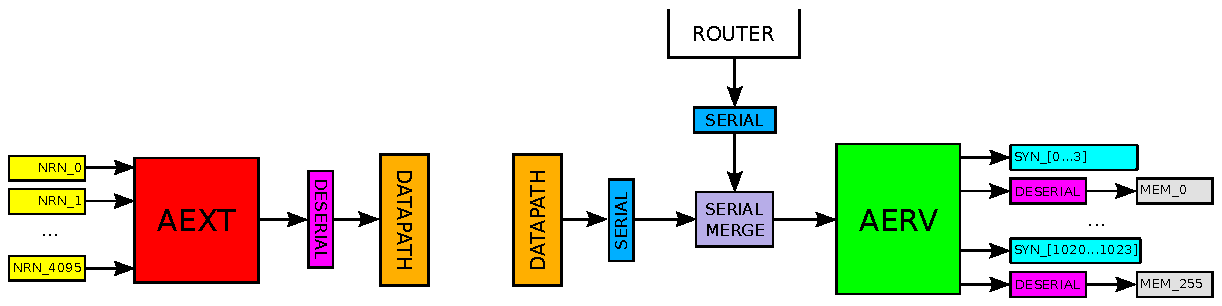
\includegraphics[width=.95\textwidth]{img/aer_system.pdf}
    \caption{Block diagram of AER system. 
    Arrows indicate the direction of data flow.}
    \label{fig:aer_system}
\end{figure}

Further, we fulfill our task subject to throughput and area constraints. Each
neuron array contains 4096 neurons. Neurons in nengo have default maximum spike 
rates between 200 and 400 spks/s. Using 400 spks/s as a worst-case
estimate (from the AER system's perspective) of each neuron's spike rate,
, we find that our system must support a throughput of at least 1.6 Mspks/s.
Currently, we're budgeting 24.5$\mu$m$^2$ per neuron for AER circuitry. This
may change depending on what Ben needs for the neuron. For area, we use a rule 
of thumb that 10 transistors take up 1.4$\mu$m$^2$. Therefore, we budget
175 transitors per neuron for the AER system.

A simplified view of the AER system is shown in Figure~\ref{fig:aer_system}.
The main components of the system are the transmitter (AEXT) and receiver (AERV).
The transmitter encodes and transmits the spikes from 4096 neurons to the 
datapath circuitry. The receiver decodes packets from the datapath circuitry 
and targets 1024 synapses and 256 memory blocks. Each synapse delivers input 
current to 4 neurons. Each memory stores the configuration bits for 4 syanpses 
and 16 neurons.

In this document, we sometimes give block diagrams, HSE, and PRS for 2-ary 
trees and 1-of-2 (dualrail) channel configurations of processes with the 
understanding that they are readily extensible to other configurations.
In practice, we use 3-ary or 4-ary tree configurations and 1-of-4 channels.

%%%%%%%%%%%%%%%%%%%%%%%%%%%%%%%%%%%%%%%%%%%%%%%%%%%%%%%%%%%%%%%%%%%%%%%%%%%%%%%
\section{Serial protocol}

The bulk of this work can be understood in context of the serial protocol
used by the receiver and transmitter. 
The transmitter simply implements this protocol on top of merging and arbitration, 
and the receiver simply implements this protocol on top of splitting.

Consider a 1-bit source and a sink connected through a buffer.

\begin{center}
    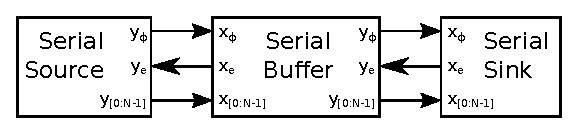
\includegraphics[width=.5\textwidth]{img/serial_protocol_block_diagram.pdf}
\end{center}

\noindent
The channels can carry four symbols:

\begin{center}
    \begin{tabular}{r|l}
    \hline
    symbol & meaning \\ \hline
    $r$ & channel has been requested \\
    0 & channel data is 0 \\
    1 & channel data is 1 \\
    $\neg r$ & channel no longer requested \\
    \hline
    \end{tabular}
\end{center}

A packet of data begins with $r$.
Following $r$ is a a sequence of 0s and 1s containing the packet data.
There is no limit on the length of the data sequence packet.
The packet ends with $\neg r$. 

\subsection{Buffer}

\noindent
The serial protocol is best understood by considering Serial Buffer.

\subsubsection*{Pseudo-code}

\begin{lstlisting}[mathescape]
Repeat {
    Wait for $r$ from the source.
    Relay $r$ from source to sink.
    While (source is not sending $\neg r$)) {
        Relay data from source to sink
    }
    Relay $\neg r$ from source to sink.
}
\end{lstlisting}

\subsubsection*{CHP}

\begin{csp}
*[[#{X=r}->Y!X?
  []#{X=0}|#{X=1}->Y!X?
  []#{X=\neg\ r}->Y!X?
 ]]
\end{csp}

\noindent
In the $\overline{X=r}$ and $\overline{X=\neg r}$ branches,
the $Y!X?$ communications are 2-phase since $r$ and $\neg r$ 
communications occur in pairs (i.e. they alternate). \\
In the $\overline{X=0}\ \vee \overline{X=1}$ branch,
the $Y!X?$ communication is 4-phase.


\subsubsection*{HSE}

\begin{hse}
*[[xr->yr+;[ye];xe+
  []x0->y0+;[~ye];xe-;[~x0];y0-;[ye];xe+
  []x1->y1+;[~ye];xe-;[~x1];y1-;[ye];xe+
  []~xr->yr-;[~ye];xe-
 ]]
\end{hse}

\noindent
The source sends the $r$ symbol by raising $xr$, and the buffer
acknowledges with $x_o\uparrow$. \\
The buffer relays the $r$ to the sink with $yr\uparrow$, and the
sink acknowledges by raising $y_i$. \\
Data from the source is relayed to the sink with standard, unpipelined,
4-phase handshakes. Note that the source is acknowledged with $x_o\downarrow$, 
and that the sink acknowledges the data by lowering $y_i$. 
The second half of the 4-phase handshakes returns the process to the state 
ready to receive data. \\
The source sends the $\neg r$ symbol by lowering $xr$, and the buffer
acknowledges with $x_o\downarrow$. \\
The buffer relays the $\neg r$ to the sink with $yr\downarrow$, and the
sink acknowledges by lowering $y_i$. \\

\noindent
The buffer's sequencing can be visualized in Figure~\ref{fig:protocol_net}.

\subsection{Source}

Serial Source outputs random data.

\subsubsection*{CHP}

\begin{csp}
*[[~u->Y!r;u+
  []u->[true->Y!0
         \|true->Y!1
         \|true->Y!\neg r;u-
         ]
 ]]
\end{csp}

\noindent
The nondeterministic selection between $true$ guards implements the random
data generation.

\subsubsection*{HSE}

\begin{hse}
*[[~u->yr+;[ye];u+
  []u->[true->y0+;[~ye];y0-;[ye]
         \|true->y1+;[~ye];y1-;[ye]
         \|true->yr-;[~ye];u-
         ]
 ]]
\end{hse}

\subsection{Sink}

Serial Sink does as sinks do.

\subsubsection*{CHP}

\begin{csp}
*[[#{X=r}->X?
  []#{X=0}|#{X=1}->X?
  []#{X=\neg r}->X?
 ]]
\end{csp}

\subsubsection*{HSE}

\begin{hse}
*[[xr->xe+
  []x0->xe-;[~x0];xe+
  []x1->xe-;[~x1];xe+
  []~xr->xe-
 ]]
\end{hse}

\begin{figure}
    \centering
    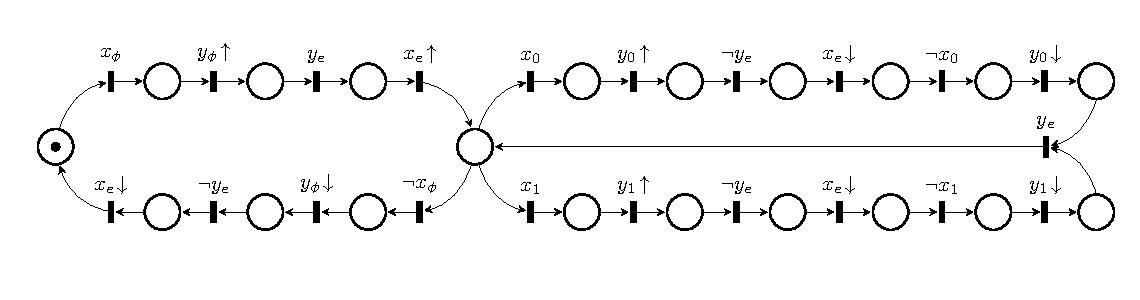
\includegraphics[width=.95\textwidth]{img/serial_protocol_petri_net.pdf}
    \caption{A petri-net of the buffer process.
Each circle is a state and each connecting line is a transition. The dot
indicates the initial state and is the token that traverses the net.
At each state, the dot picks one of the outgoing transitions to execute
and follows it to the next state. The left side of the net is the control
portion of the sequence. The right side of the net is the data transfer
portion of the sequence.}
    \label{fig:protocol_net}
\end{figure}

%%%%%%%%%%%%%%%%%%%%%%%%%%%%%%%%%%%%%%%%%%%%%%%%%%%%%%%%%%%%%%%%%%%%%%%%%%%%%%%
\section{Transmitter (AEXT)}

The transmitter is internally organized as a 4-ary tree consisting of intermediate
nodes (NODE) and leaf nodes (LEAF).
\begin{center}
    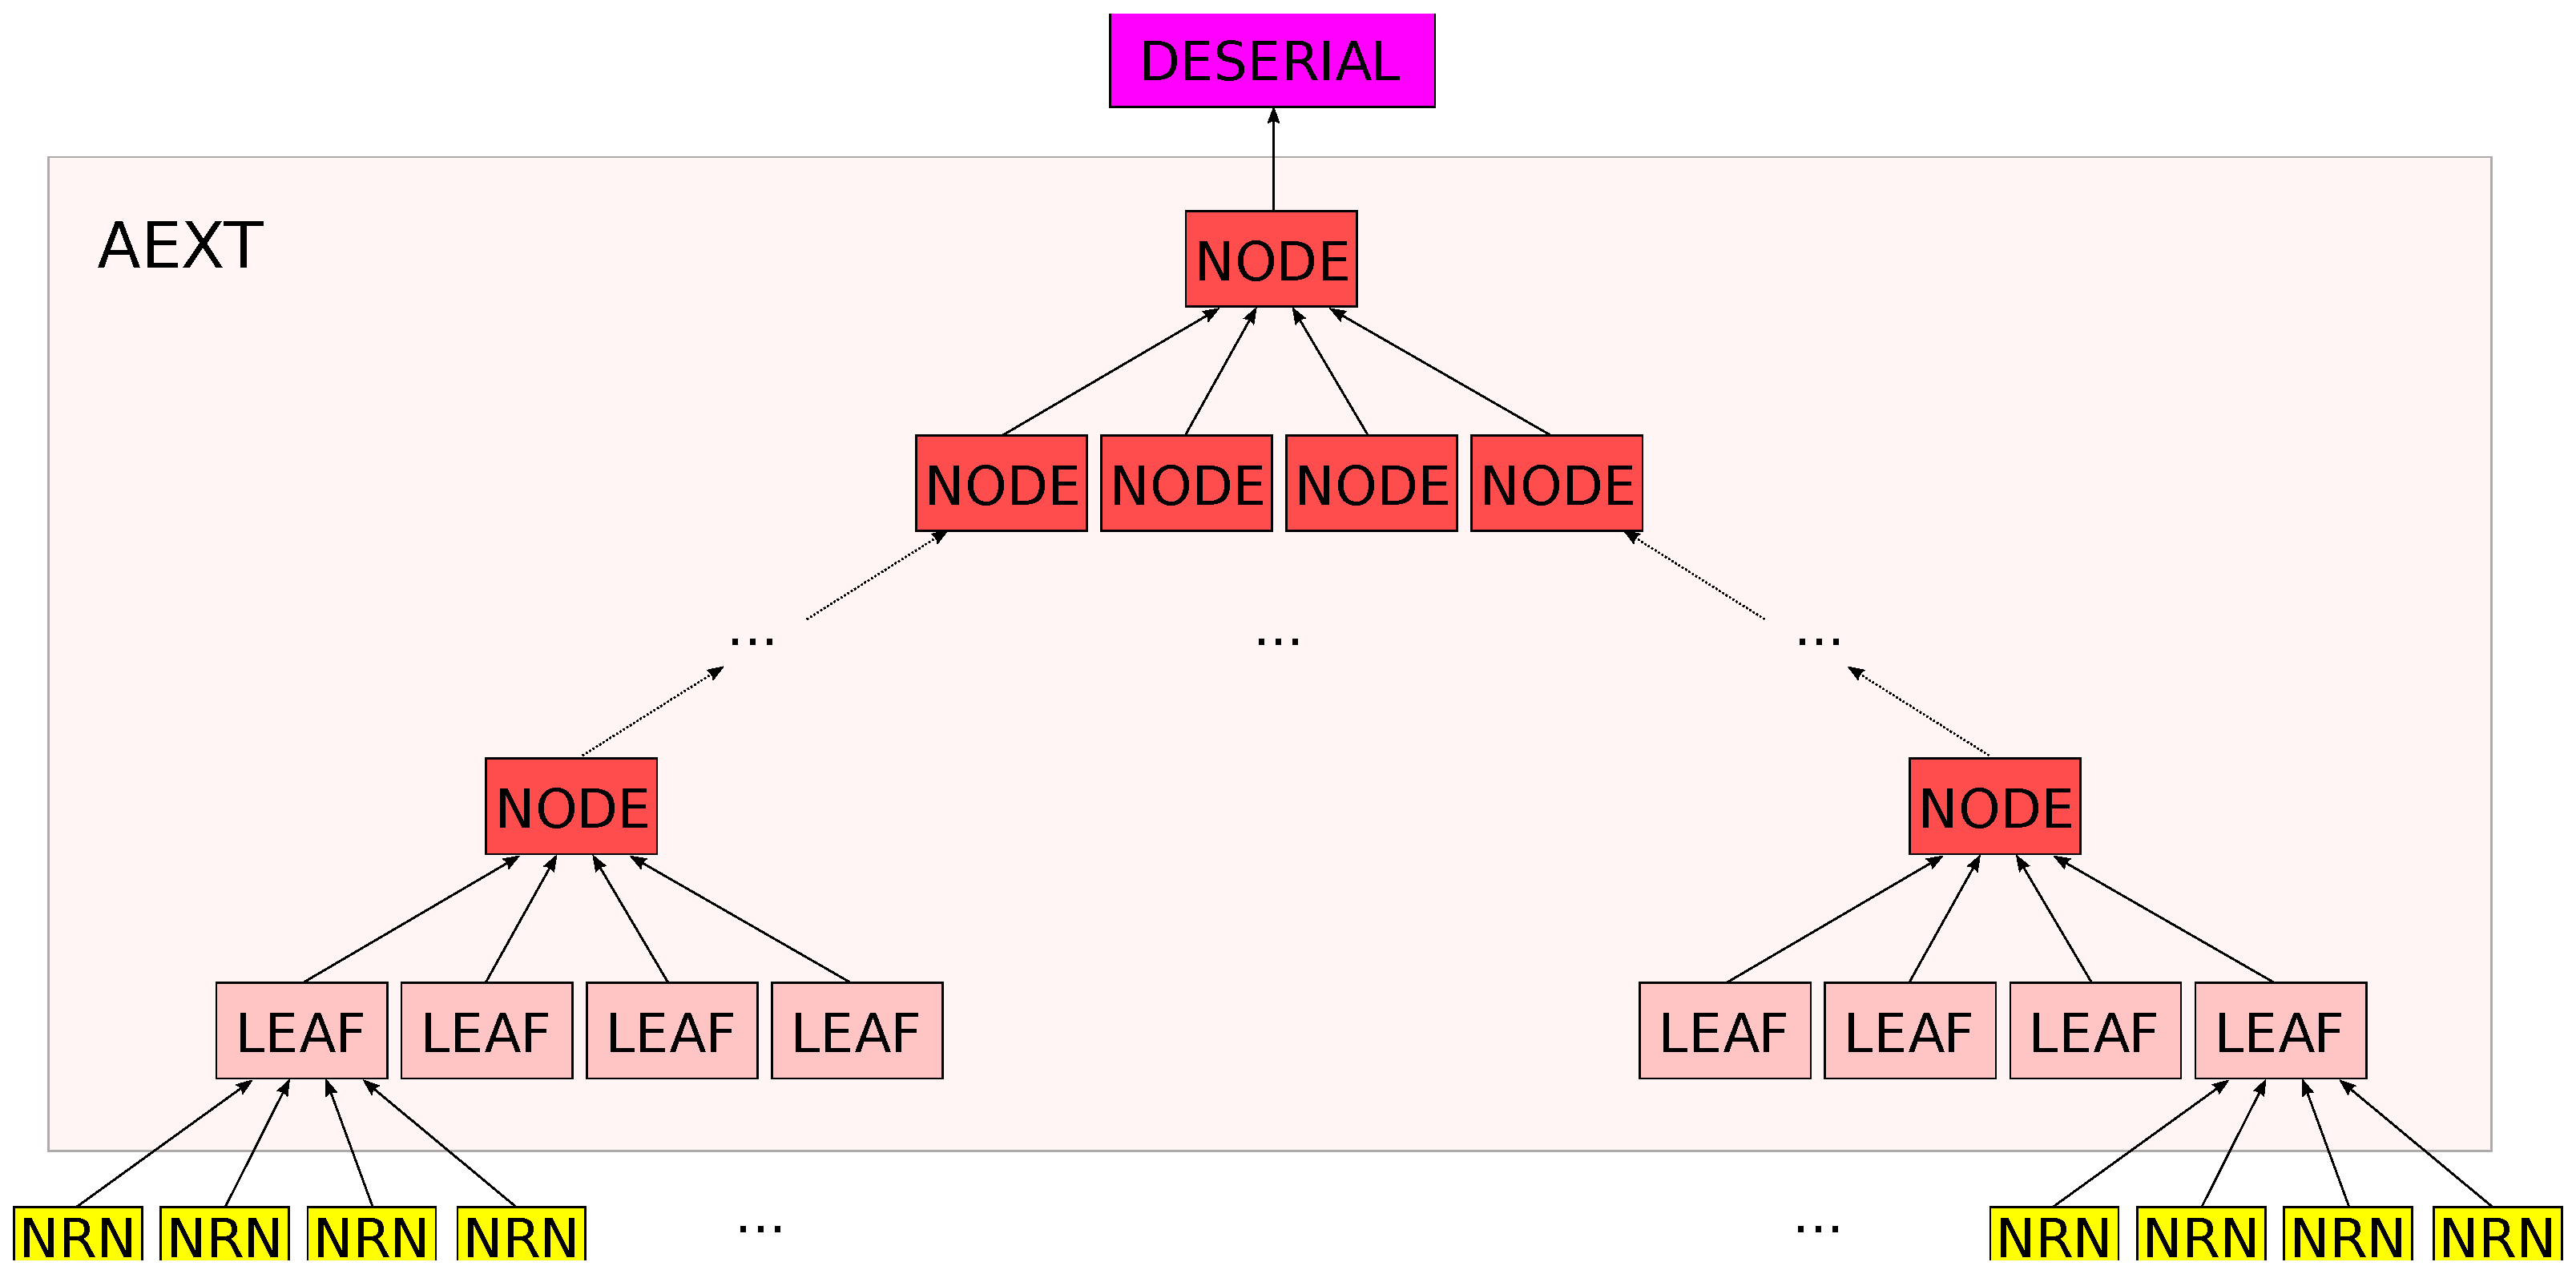
\includegraphics[width=.7\textwidth]{img/aext.pdf}
\end{center}
Neurons (NRNs) connect to the transmitter at the leaves of the tree.
When a neuron spikes, a packet travels from the attached leaf to the root of 
the tree. Neurons spike asynchronously and so may signal the transmitter at 
arbitrary times. We thus use an arbiter in each LEAF and NODE to sequence the 
incoming spike packets into a combined output packet stream. Further, at each 
LEAF and NODE, a spike packet is prepended with a word indicating which 
branch it came from.

%%%%%%%%%%%%%%%%%%%%%%%%%%%%%%%%%%%%%%%%%%%%%%%%%%%%%%%%%%%%%%%%%%%%%%%%%%%%%%%
\subsection{Neuron (NRN) \label{sec:AEXT_NRN}}

From the perspective of the transmitter, neurons simply transmit $r$ to 
emit a spike and $\neg r$ after reset.

\subsubsection*{CHP}

\begin{csp}
*[X!r;X!\neg r]
\end{csp}

\subsubsection*{HSE}

\begin{hse}
*[xr+;[xa];xr-;[~xa]]
\end{hse}

\noindent
The HSE implements the two CHP communications using a pair of 2-phase handshakes.

\noindent
With the neuron's internal signals,

\begin{hse}
*[[~_SPK];REQ+;[ACK];[_SPK];REQ-;[~ACK]]
\end{hse}

\begin{prs2}
~_SPK & ~ACK -> REQ+
_SPK & ACK -> REQ-
\end{prs2}

%%%%%%%%%%%%%%%%%%%%%%%%%%%%%%%%%%%%%%%%%%%%%%%%%%%%%%%%%%%%%%%%%%%%%%%%%%%%%%%
\subsection{AEXT LEAF \label{sec:AEXT_LEAF}}

The LEAF node receives spikes from its attached neurons and initiates spike
packets to send up the tree. The input/output ports are shown as follows:

\begin{center}
  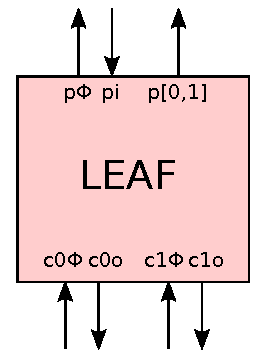
\includegraphics[width=.16\textwidth]{img/aext_leaf.pdf}
\end{center}

\noindent
As mentioned in Section~\ref{sec:intro}, although
we give diagrams and code for a binary tree and 1-of-2 words for the sake of 
compactness, the design uses a 4-ary tree and 1-of-4 words.

\subsubsection*{Pseudo-code}

\begin{lstlisting}[mathescape]
Repeat {
    Wait for and arbitrate between $r$ from the neurons.
    Relay $r$ from the arbiter-selected neuron to parent.
    Send 0, 1, 2, or 3 to the parent indicating which neuron was selected.
    Relay $\neg r$ from the selected neuron to the parent.
}
\end{lstlisting}

\subsubsection*{CHP}

\begin{csp}
*[[#{C0=r}->P!C0?;P!0;P!C0?
  \|#{C1=r}->P!C1?;P!1;P!C0?
 ]]
\end{csp}

\noindent
Matching the CHP to the psuedo-code, the nondeterministic selection and 
probes implement the wait and arbitrate between neurons. \\
Traversing the first branch, $P!C0?$ relays $r$ from neuron to parent. \\
$P!0$ sends $0$ to the parent to indicate the selected neuron. \\
The second $P!C0?$ relays $\neg r$ from neuron to parent.

\subsubsection*{HSE}

We implement the HSE

\begin{hse}
*[[c0r->c0+;[~c0r];c0-
  \|c1r->c1+;[~c1r];c1-
 ]]

*[[c0->pr+;[pe];u0+;
    p0+;[~pe];v+;c0a+;[~c0];p0-;[pe];
    pr-;[~pe];u0-;c0a-,v-
  []c1->pr+;[pe];u1+;
    p1+;[~pe];v+;c1a+;[~c1];p1-;[pe];
    pr-;[~pe];u1-;c1a-,v-
 ]]
\end{hse}

\noindent
To get there, we start by directly translating the CHP:

\begin{hse}
*[[c0r->pr+;[pe];c0e+;
    p0+;[~pe];p0-;[pe];
    [~c0r];pr-;[~pe];c0e-
  \|c1r->pr+;[pe];c1e+;
    p1+;[~pe];p1-;[pe];
    [~c1r];pr-;[~pe];c1e-
 ]]
\end{hse}

\noindent
To match the HSE to the CHP, consider the first branch of the nondeterministic
selection: 

$c0r\rightarrow\ r\uparrow;\texttt{[}pe\texttt{]};c0_o$ implements 
$\overline{C0=r}\longrightarrow P!C0?$ with 2-phase communications that
pair with the 2-phase communications at the end of the branch.

$p0\uparrow;\texttt{[}\neg pe\texttt{]};p0\downarrow;\texttt{[}pe\texttt{]}$ implements $P!0$ with a 4-phase communication.

$\texttt{[}\neg c0r\texttt{]};pr\downarrow;\texttt{[}\neg pe\texttt{]};c0o\downarrow$ implements $P!C0$ with 2-phase communications that pair with the 
2-phase communications at the beginning of the branch. \\

\noindent
The states immediately before and after the second communication are 
indistinguishable, so we overlap the first and the third communications into 
the second communication.

\begin{hse}
*[[c0r->pr+;[pe];
    p0+;[~pe];\red{c0e+;[~c0r]};p0-;[pe];
    pr-;[~pe];c0e-
  \|c1r->pr+;[pe];
    p1+;[~pe];\red{c1e+;[~c1r]};p1-;[pe];
    pr-;[~pe];c1e-
 ]]
\end{hse}

\noindent
Since we have ready-made N-way arbiters, we introduce state variables $c[0,1]$
to represent the arbitration.

\begin{hse}
*[[c0r->\red{c0+};pr+;[pe];
    p0+;[~pe];c0e+;[~c0r];\red{c0-};p0-;[pe];
    pr-;[~pe];c0e-
  \|c1r->\red{c1+};pr+;[pe];
    p1+;[~pe];c1e+;[~c1r];\red{c1-};p1-;[pe];
    pr-;[~pe];c1e-
 ]]
\end{hse}

\noindent
and break out the nondeterministic selection into a separate, arbitration process.

\begin{hse}
*[[\red{c0r->c0+;[~c0r];c0-}
  \|\red{c1r->c1+;[~c1r];c1-}
 ]]

*[[\red{c0}->pr+;[pe];
    p0+;[~pe];c0e+;[\red{~c0}];p0-;[pe];
    pr-;[~pe];c0e-
  []\red{c1}->pr+;[pe];
    p1+;[~pe];c1e+;[\red{~c1}];p1-;[pe];
    pr-;[~pe];c1e-
 ]]
\end{hse}

\noindent
However, note that the arbitration process is free to select a different branch
as soon as one branch completes. For example, after $c0\!\downarrow$ compeletes,
the arbitration process is free to execute $c1\!\uparrow$ should $c1r$ be high.
Therefore, we add state variable $v$ to preserve the mutual exclusion in the
mutually exclusive selection process.

\begin{hse}
*[[c0r->c0+;[~c0r];c0-
  \|c1r->c1+;[~c1r];c1-
 ]]

*[[c0->pr+;[pe];
    p0+;[~pe];\red{v+};c0e+;[~c0];p0-;[pe];
    pr-;[~pe];c0e-,\red{v-}
  []c1->pr+;[pe];
    p1+;[~pe];\red{v+};c1e+;[~c1];p1-;[pe];
    pr-;[~pe];c1e-,\red{v-}
 ]]
\end{hse}

\noindent
Since $v\!\uparrow$ occurs before acknowledging the neurons with $c0_o\!\uparrow$
or $c1_o\!\uparrow$, we can use $v$ to exclude the non-selected branches.

\noindent
Finally, to make the $p[0,1]$ and $c[0,1]_o$ gates combinational and overall 
reduce transistor count, we introduce state variables $u[0,1]$.

\begin{hse}
*[[c0r->c0+;[~c0r];c0-
  \|c1r->c1+;[~c1r];c1-
 ]]

*[[c0->pr+;[pe];\red{u0+}
    p0+;[~pe];v+;c0e+;[~c0];p0-;[pe];
    pr-;[~pe];\red{u0-};c0e-,v-
  []c1->pr+;[pe];\red{u1+}
    p1+;[~pe];v+;c1e+;[~c1];p1-;[pe];
    pr-;[~pe];\red{u1-};c1e-,v-
 ]]
\end{hse}

\noindent
which completes our expansion.

\subsubsection*{PRS}

The $c0$ and $c1$ state variables are the outputs of a standard N-way arbiter
with inputs $c0_i$ and $c1_i$.

\begin{prs2}
(c0 | c1) & ~v -> pr+
pe & v -> pr-
\end{prs2}

\begin{prs2}
c0 & pe & ~v -> u0+
~c0 & ~pr & ~pe -> u0-

c1 & pe & ~v -> u1+
~c1 & ~pr & ~pe -> u1-
\end{prs2}

\noindent
The $\neg c[0,1]$ in the pulldowns eliminate an isochronic fork to allow for
bubble-reshuffling.

\begin{prs2}
(u0 | u1) & ~pe -> v+
~u0 & ~u1 -> v-
\end{prs2}

\begin{prs2}
u0 & c0 -> p0+
~u0 | ~c0 -> p0-

u1 & c1 -> p1+
~u1 | ~c1 -> p1-
\end{prs2}

\begin{prs2}
u0 & v -> c0e+
~u0 | ~v -> c0e-

u1 & v -> c1e+
~u1 | ~v -> c1e-
\end{prs2}

\noindent
4-ary approximate accounting:

\begin{center}
    \begin{tabular}{|r|l|l|}
    \hline
    rule & transistor count & comments \\ \hline
    $c[0,1,2,3]$ & 92 & 4-way unpipelined arbiter \\ \hline
    $pr$ & 11 & \\ \hline
    $u[0,1,2,3]$ & 40 & \\ \hline
    $v$ & 13 & \\ \hline
    $p[0,1,2,3]$ & 16 & \\ \hline
    $c[0,1,2,3]_o$ & 16 & \\ \hline
    \hline total & 188 & \\ \hline
    \end{tabular}
\end{center}

\subsubsection*{CMOS-implementable PRS}

\begin{prs2}
~v -> _v+
v -> _v-

~_v -> __v+
_v -> __v-
\end{prs2}

\begin{prs2}
~c0 -> _c0+
c0 -> _c0-

~c1 -> _c1+
c1 -> _c1-
\end{prs2}

\begin{prs2}
(~_c0 | ~_c1) & ~__v -> pr+
pe & __v -> pr-
\end{prs2}

\begin{prs2}
~_c0 -> __c0+
_c0 -> __c0-

~_c1 -> __c1+
_c1 -> __c1-
\end{prs2}

\begin{prs2}
__c0 & pe & _v -> _u0-
~__c0 & ~pr & ~pe -> _u0+

__c1 & pe & _v -> _u1-
~__c1 & ~pr & ~pe -> _u1+
\end{prs2}

\begin{prs2}
(~_u0 | ~_u1) & ~pe -> v+
_u0 & _u1 -> v-
\end{prs2}

\begin{prs2}
~_u0 & ~_c0 -> p0+
_u0 | _c0 -> p0-

~_u1 & ~_c1 -> p1+
_u1 | _c1 -> p1-
\end{prs2}

\begin{prs2}
~_u0 & ~_v -> c0e+
_u0 | _v -> c0e-

~_u1 & ~_v -> c1e+
_u1 | _v -> c1e-
\end{prs2}

\noindent
4-ary approximate accounting:

\begin{center}
    \begin{tabular}{|r|l|l|}
    \hline
    rule & transistor count & comments \\ \hline
    $\_v$ & 2 & \\ \hline
    $\_\_v$ & 2 & \\ \hline
    $c[0,1,2,3]$ & 92 & 4-way unpipelined arbiter \\ \hline
    $\_c[0,1,2,3]$ & 8 & \\ \hline
    $\_pr$ & 11 & \\ \hline
    $\_\_c[0,1,2,3]$ & 8 & \\ \hline
    $\_u[0,1,2,3]$ & 40 & \\ \hline
    $\_v$ & 13 & \\ \hline
    $p[0,1,2,3]$ & 16 & \\ \hline
    $c[0,1,2,3]_o$ & 16 & \\ \hline
    \hline total & 208 & \\ \hline
    \end{tabular}
\end{center}

%%%%%%%%%%%%%%%%%%%%%%%%%%%%%%%%%%%%%%%%%%%%%%%%%%%%%%%%%%%%%%%%%%%%%%%%%%%%%%%
\subsection{AEXT NODE \label{sec:AEXT_NODE}}

The intermediate node propagates spike packets from its children to its parent.
It prepends a word to each packet indicating which child the packet is from. 
The input/output ports are shown as follows:

\begin{center}
  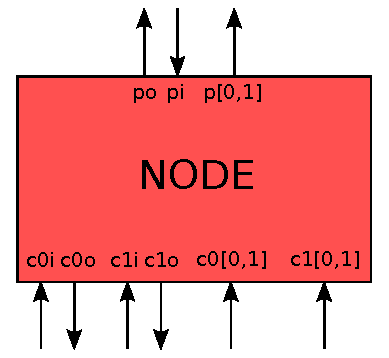
\includegraphics[width=.25\textwidth]{img/aext_node.pdf}
\end{center}

\subsubsection*{Pseudo-code}

\begin{lstlisting}[mathescape]
Repeat {
    Wait for and arbitrate between $r$ from the children.
    Relay $r$ from the arbiter-selected child to parent.
    Send 0, 1, 2, or 3 to the parent indicating which child was selected.
    While (selected child is not sending $\neg r$) {
        Relay data from the selected child to parent
    }
    Relay $\neg r$ from the selected child to the parent.
}
\end{lstlisting}

\subsubsection*{CHP}

\begin{csp}
*[[#{C0=r}->P!C0?;P!0;[#{C0=\neg r}->P!C0?]
  \|#{C1=r}->P!C1?;P!1;[#{C1=\neg r}->P!C1?]
 ]]

*[[(#{C0=0}|#{C0=1})->P!C0?
  [](#{C1=0}|#{C1=1})->P!C1?
 ]]
\end{csp}

\noindent
Matching the CHP to the psuedo-code, the nondeterministic selection and 
probes in the first process implement the wait and arbitrate between children. \\
Traversing the first process' first branch, $P!C0?$ relays $r$ to the parent. \\
$P!0$ sends $0$ to the parent to indicate the selected child. \\
Next, we wait for $\overline{C0=\neg r}$, which implements the while-loop 
condition. \\
While the top process waits for $\neg r$, the bottom process relays 
data from the children to the parent. \\
A child following the serial protocol only sends data after having 
its $r$ communication completed. Therefore the arbitration in
the top process ensures that branches in the bottom process are mutually 
exclusive. \\
Finally, when $\neg r$ arrives, we return to the top process and relay
$\neg r$ with $P!C0?$. \\


\subsubsection*{HSE}

We implement the HSE

\begin{hse}
*[[c0r->c0+;[~c0r];c0-
  \|c1r->c1+;[~c1r];c1-
 ]]

*[[c0->pr+;[pe];w0+;
    p0+[~pe];u+;w0-;p0-;[pe];c0e+;
    [~c0];pr-;[~pe];c0e-;u-
  []c1->pr+;[pe];w1+;
    p1+;[~pe];u+;w1-;p1-;[pe];c1e+;
    [~c1];pr-;[~pe];c1e-;u-
 ]]
\end{hse}

\begin{hse}
*[[c00->p0+;[~pe];c0e-;[~c00];p0-;[pe];c0e+
  []c01->p1+;[~pe];c1e-;[~c01];p1-;[pe];c1e+
  []c10->p0+;[~pe];c0e-;[~c10];p0-;[pe];c0e+
  []c11->p1+;[~pe];c1e-;[~c11];p1-;[pe];c1e+
 ]]
\end{hse}

\noindent
To get there, we first directly translate the CHP.

\begin{hse}
*[[c0r->pr+;[pe];c0e+;
    p0+;[~pe];p0-;[pe];
    [~c0r];pr-;[~pe];c0e-
  \|c1r->pr+;[pe];c1e+;
    p1+;[~pe];p1-;[pe];
    [~c1r];pr-;[~pe];c1e-
 ]]
\end{hse}

\begin{hse}
*[[c00->p0+;[~pe];c0e-;[~c00];p0-;[pe];c0e+
  []c01->p1+;[~pe];c1e-;[~c01];p1-;[pe];c1e+
  []c10->p0+;[~pe];c0e-;[~c10];p0-;[pe];c0e+
  []c11->p1+;[~pe];c1e-;[~c11];p1-;[pe];c1e+
 ]]
\end{hse}

\noindent
The top process is the same as the initial LEAF HSE. The bottom process is the 
standard, unpipelined 4-phase handshake expansion of relaying data from the 
children to the parent.

\noindent
The child can send data as soon as $c[0,1]_o\!\uparrow$ completes.
To ensure that we prepend a word indicating which child was selected before
the child sends data, we overlap the $P!C[0,1]?$ communications relaying
$r$ to the parent across the $P![0,1]$ communications.

\begin{hse}
*[[c0r->pr+;[pe];
    p0+;[~pe];p0-;[pe];\red{c0e+;}
    [~c0r];pr-;[~pe];c0e-
  \|c1r->pr+;[pe];
    p1+;[~pe];p1-;[pe];\red{c1e+;}
    [~c1r];pr-;[~pe];c1e-
 ]]
\end{hse}

\begin{hse}
*[[c00->p0+;[~pe];c0e-;[~c00];p0-;[pe];c0e+
  []c01->p1+;[~pe];c1e-;[~c01];p1-;[pe];c1e+
  []c10->p0+;[~pe];c0e-;[~c10];p0-;[pe];c0e+
  []c11->p1+;[~pe];c1e-;[~c11];p1-;[pe];c1e+
 ]]
\end{hse}

\noindent
The states immediately before and after the $P![0,1]$ communications are
indistinguishable, so we introduce state variables $u0$ and $u1$.

\begin{hse}
*[[c0r->pr+;[pe];\red{u0+};
    p0+;[~pe];\red{u0-};p0-;[pe];c0e+;
    [~c0r];pr-;[~pe];c0e-
  \|c1r->pr+;[pe];\red{u1+};
    p1+;[~pe];\red{u1-};p1-;[pe];c1e+;
    [~c1r];pr-;[~pe];c1e-
 ]]
\end{hse}

\begin{hse}
*[[c00->p0+;[~pe];c0e-;[~c00];p0-;[pe];c0e+
  []c01->p1+;[~pe];c1e-;[~c01];p1-;[pe];c1e+
  []c10->p0+;[~pe];c0e-;[~c10];p0-;[pe];c0e+
  []c11->p1+;[~pe];c1e-;[~c11];p1-;[pe];c1e+
 ]]
\end{hse}

\noindent
Since we have ready-made N-way arbiters, we introduce state variables $c[0,1]$ 
to represent the arbitration.

\begin{hse}
*[[c0r->\red{c0+};pr+;[pe];u0+
    p0+;[~pe];u0-;p0-;[pe];c0e+;
    [~c0r];\red{c0-};pr-;[~pe];c0e-
  \|c1r->\red{c1+};pr+;[pe];u1+
    p1+;[~pe];u1-;p1-;[pe];c1e+;
    [~c1r];\red{c1-};pr-;[~pe];c1e-
 ]]
\end{hse}

\begin{hse}
*[[c00->p0+;[~pe];c0e-;[~c00];p0-;[pe];c0e+
  []c01->p1+;[~pe];c1e-;[~c01];p1-;[pe];c1e+
  []c10->p0+;[~pe];c0e-;[~c10];p0-;[pe];c0e+
  []c11->p1+;[~pe];c1e-;[~c11];p1-;[pe];c1e+
 ]]
\end{hse}

\noindent
and break out the nondeterministic selection into a separate, arbitration process.

\begin{hse}
*[[\red{c0r->c0+;[~c0r];c0-}
  \|\red{c1r->c1+;[~c1r];c1-}
 ]]

*[[\red{c0}->pr+;[pe];u0+;
    p0+[~pe];u0-;p0-;[pe];c0e+;
    [\red{~c0}];pr-;[~pe];c0e-
  []\red{c1}->pr+;[pe];u1+;
    p1+;[~pe];u1-;p1-;[pe];c1e+;
    [\red{~c1}];pr-;[~pe];c1e-
 ]]
\end{hse}

\begin{hse}
*[[c00->p0+;[~pe];c0e-;[~c00];p0-;[pe];c0e+
  []c01->p1+;[~pe];c1e-;[~c01];p1-;[pe];c1e+
  []c10->p0+;[~pe];c0e-;[~c10];p0-;[pe];c0e+
  []c11->p1+;[~pe];c1e-;[~c11];p1-;[pe];c1e+
 ]]
\end{hse}

\noindent
As in AEXT LEAF, the arbitration process is free to select a different branch
as soon as one branch completes. Therefore, we add state variable $v$ to preserve the mutual exclusion in the mutually exclusive selection.

\begin{hse}
*[[c0r->c0+;[~c0r];c0-
  \|c1r->c1+;[~c1r];c1-
 ]]

*[[c0->pr+;[pe];u0+;
    p0+;[~pe];\red{v+};u0-;p0-;[pe];c0e+;
    [~c0];pr-;[~pe];c0e-;\red{v-}
  []c1->pr+;[pe];u0+;
    p1+;[~pe];\red{v+};u1-;p1-;[pe];c1e+;
    [~c1];pr-;[~pe];c1e-;\red{v-}
 ]]
\end{hse}

\begin{hse}
*[[c00->p0+;[~pe];c0e-;[~c00];p0-;[pe];c0e+
  []c01->p1+;[~pe];c1e-;[~c01];p1-;[pe];c1e+
  []c10->p0+;[~pe];c0e-;[~c10];p0-;[pe];c0e+
  []c11->p1+;[~pe];c1e-;[~c11];p1-;[pe];c1e+
 ]]
\end{hse}

\noindent
which completes our expansion.

\subsubsection*{PRS}

\begin{prs2}
~u & (c0 | c1) -> pr+
(c0o & ~c0) | (c1o & ~c1) -> pr-
\end{prs2}

\begin{prs2}
c0 & pe & ~u -> w0+
u -> w0-

c1 & pe & ~u -> w1+
u -> w1-
\end{prs2}

\begin{prs2}
(w0 | w1) & ~pe -> u+
~c0o & ~c1o & ~pr -> u-
\end{prs2}

\begin{prs2}
c0 & u & pe & ~c1o -> c0e+
~pe -> c0e-

c1 & u & pe ~c0o -> c1e+
~pe -> c1e-
\end{prs2}

\begin{prs2}
c00 | c10 | w0 -> p0+
~c00 & ~c10 & ~w0 -> p0-

c01 | c11 | w1 -> p1+
~c01 & ~c11 & ~w1 -> p1-
\end{prs2}

\noindent
4-ary approximate accounting:

\begin{center}
    \begin{tabular}{|r|l|l|}
    \hline
    rule & transistor count & comments \\ \hline
    $c[0,1,2,3]$ & 92 & 4-way unpipelined arbiter \\ \hline
    $p_o$ & 19 & \\ \hline
    $w[0,1,2,3]$ & 32 & \\ \hline
    $u$ & 10 & \\ \hline
    $c[0,1,2,3]_o$ & 44 & \\ \hline
    $p[0,1,2,3]$ & 40 & \\ \hline
    \hline total & 237 & \\ \hline
    \end{tabular}
\end{center}

\subsubsection*{CMOS-implementable PRS}

\begin{prs2}
_u & (c0 | c1) -> _pr-
(~_c0o & ~c0) | (~_c1o & ~c1) -> _pr+

~_pr -> pr+
_pr -> pr-
\end{prs2}

\begin{prs2}
c0 & pe & _u -> _w0-
~_u -> _w0+

c1 & pe & _u -> _w1-
~_u -> _w1+
\end{prs2}

\begin{prs2}
(~_w0 | ~_w1) & ~pe -> u+
_c0o & _c1o & _pr -> u-

~u -> _u+
u -> _u-
\end{prs2}

\begin{prs2}
c0 & u & pe & _c1o -> _c0e-
~pe -> _c0e+

c1 & u & pe _c0o -> _c1e-
~pe -> _c1e+
\end{prs2}

\begin{prs2}
~_c0o -> c0e+
_c0o -> c0e-

~_c1o -> c1e+
_c1o -> c1e-
\end{prs2}

\begin{prs2}
~_c00 | ~_c10 | ~_w0 -> p0+
_c00 & _c10 & _w0 -> p0-

~_c01 | ~_c11 | ~_w1 -> p1+
_c01 & _c11 & _w1 -> p1-
\end{prs2}

\begin{prs2}
~p0 -> _p0+
p0 -> _p0-

~p1 -> _p1+
p1 -> _p1-
\end{prs2}

\noindent
Note that the root NODE does not create $\_p[0,1]$.
We simply present a normal-sense $pe$, $pr$, and $p[0,1]$ interface to the environment.

\noindent
4-ary accounting:

\begin{center}
    \begin{tabular}{|r|l|l|}
    \hline
    rule & transistor count & comments \\ \hline
    $c[0,1,2,3]$ & 92 & 4-way unpipelined arbiter \\ \hline
    $\_pr$ & 13 & staticized by $pr$ \\ \hline
    $pr$ & 4 & staticizes $\_pr$ \\ \hline
    $\_w[0,1,2,3]$ & 32 & \\ \hline
    $u$ & 10 & staticized by $\_u$ \\ \hline
    $\_u$ & 4 & staticizes $u$ \\ \hline
    $\_c[0,1,2,3]_o$ & 36 & staticized by $c[0,1,2,3]_o$ \\ \hline
    $c[0,1,2,3]_o$ & 16 & staticizes $\_c[0,1,2,3]_o$\\ \hline
    $p[0,1,2,3]$ & 40 & \\ \hline
    $\_p[0,1,2,3]$ & 8 & \\ \hline
    \hline total & 255 & \\ \hline
    \end{tabular}
\end{center}

%%%%%%%%%%%%%%%%%%%%%%%%%%%%%%%%%%%%%%%%%%%%%%%%%%%%%%%%%%%%%%%%%%%%%%%%%%%%%%%
\subsection{Neuron Buffer (NRN\_BUF) \label{sec:AEXT_NRN_BUF}}

The refractory period of the neuron can last up to milliseconds, so we need to
add some buffering between the neuron and the transmitter to prevent a neuron
from locking up the whole transmitter tree during its refractory period.

We assume that neuron contains a C-element at its output already.

\subsubsection{HSE}

\begin{hse}
*[[xr];yr+;[ye];xe+;yr-;[~ye&~xr];xe-]
\end{hse}

\subsubsection{PRS}

\begin{prs2}
xr & ~xe -> yr+
~xr | xe -> yr-

ye -> xe+
~xr & ~ye -> xe-
\end{prs2}

\noindent
approximate accounting:

\begin{center}
    \begin{tabular}{|r|l|l|}
    \hline
    rule & transistor count & comments \\ \hline
    $yr$ & 4 & \\ \hline
    $x_o$ & 7 & \\ \hline
    \hline total & 11 & \\ \hline
    \end{tabular}
\end{center}

\subsubsection{CMOS-implementable PRS}

\begin{prs2}
xr & _xo -> _yr-
~xr | ~_xo -> _yr+

ye -> _xe-
~xr & ~ye -> _xe+
\end{prs2}

\begin{prs2}
~_xo -> __xe+
_xo -> __xe-
\end{prs2}

\noindent
accounting:

\begin{center}
    \begin{tabular}{|r|l|l|}
    \hline
    rule & transistor count & comments \\ \hline
    $yr$ & 4 & \\ \hline
    $\_x_o$ & 3 & staticized by $\_\_x_o$ \\ \hline
    $\_\_x_o$ & 4 & staticizes $x_o$ \\ \hline
    \hline total & 11 & \\ \hline
    \end{tabular}
\end{center}

%%%%%%%%%%%%%%%%%%%%%%%%%%%%%%%%%%%%%%%%%%%%%%%%%%%%%%%%%%%%%%%%%%%%%%%%%%%%%%%
\section{Receiver (AERV) \label{sec:AERV}}

Like the transmitter, the receiver is internally organized as a 4-ary tree.
However, the receiver uses a single kind of node (NODE).
The receiver's task is complicated by the need to deliver specific kinds
of spikes (excitatory and inibitory) to the synapses as well as memory 
configuration packets to the syanpse and neuron memory blocks.
The receiver tree structure is dictated by its interface with the synapses and 
memory blocks. The NODEs at the leaves of the receiver have three output ports. 
Two ports send spike packets to 2 synapses (8 neurons) each. The third port
communicates with a memory block for the 4 synapses (16 neurons).
Consolidating the memory for 4 synapses (16 neurons) reduces the overhead of 
deserializers. Dedicating a port of the NODE to memory allow us to further 
reduce overhead by using 1-of-4 coding in the deserializer 
(see Section~\ref{sec:DESERIAL}):

\begin{center}
  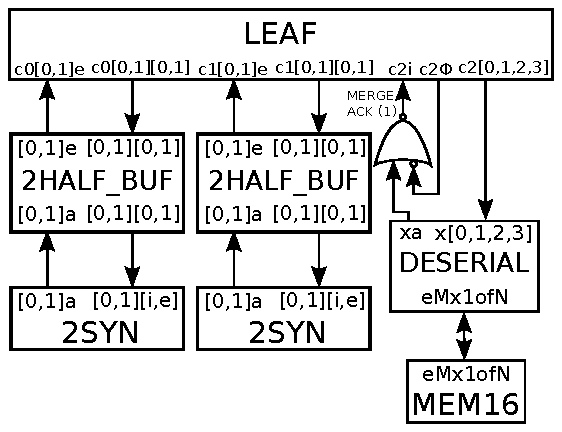
\includegraphics[width=.5\textwidth]{img/recv_nrn_interface_2syn2_1mem16.pdf}
\end{center}

\noindent
The receiver tree structure is given as follows:

\begin{center}
    \begin{tabular}{cc}
        1 NODE & \\
        4 NODE & \\
        16 NODE & \\
        64 NODE & \\
        256 NODE(3) & \\
        512 SYN2 & 256 DESERIAL \\
        & 256 MEM16 \\
    \end{tabular}
\end{center}

\begin{center}
  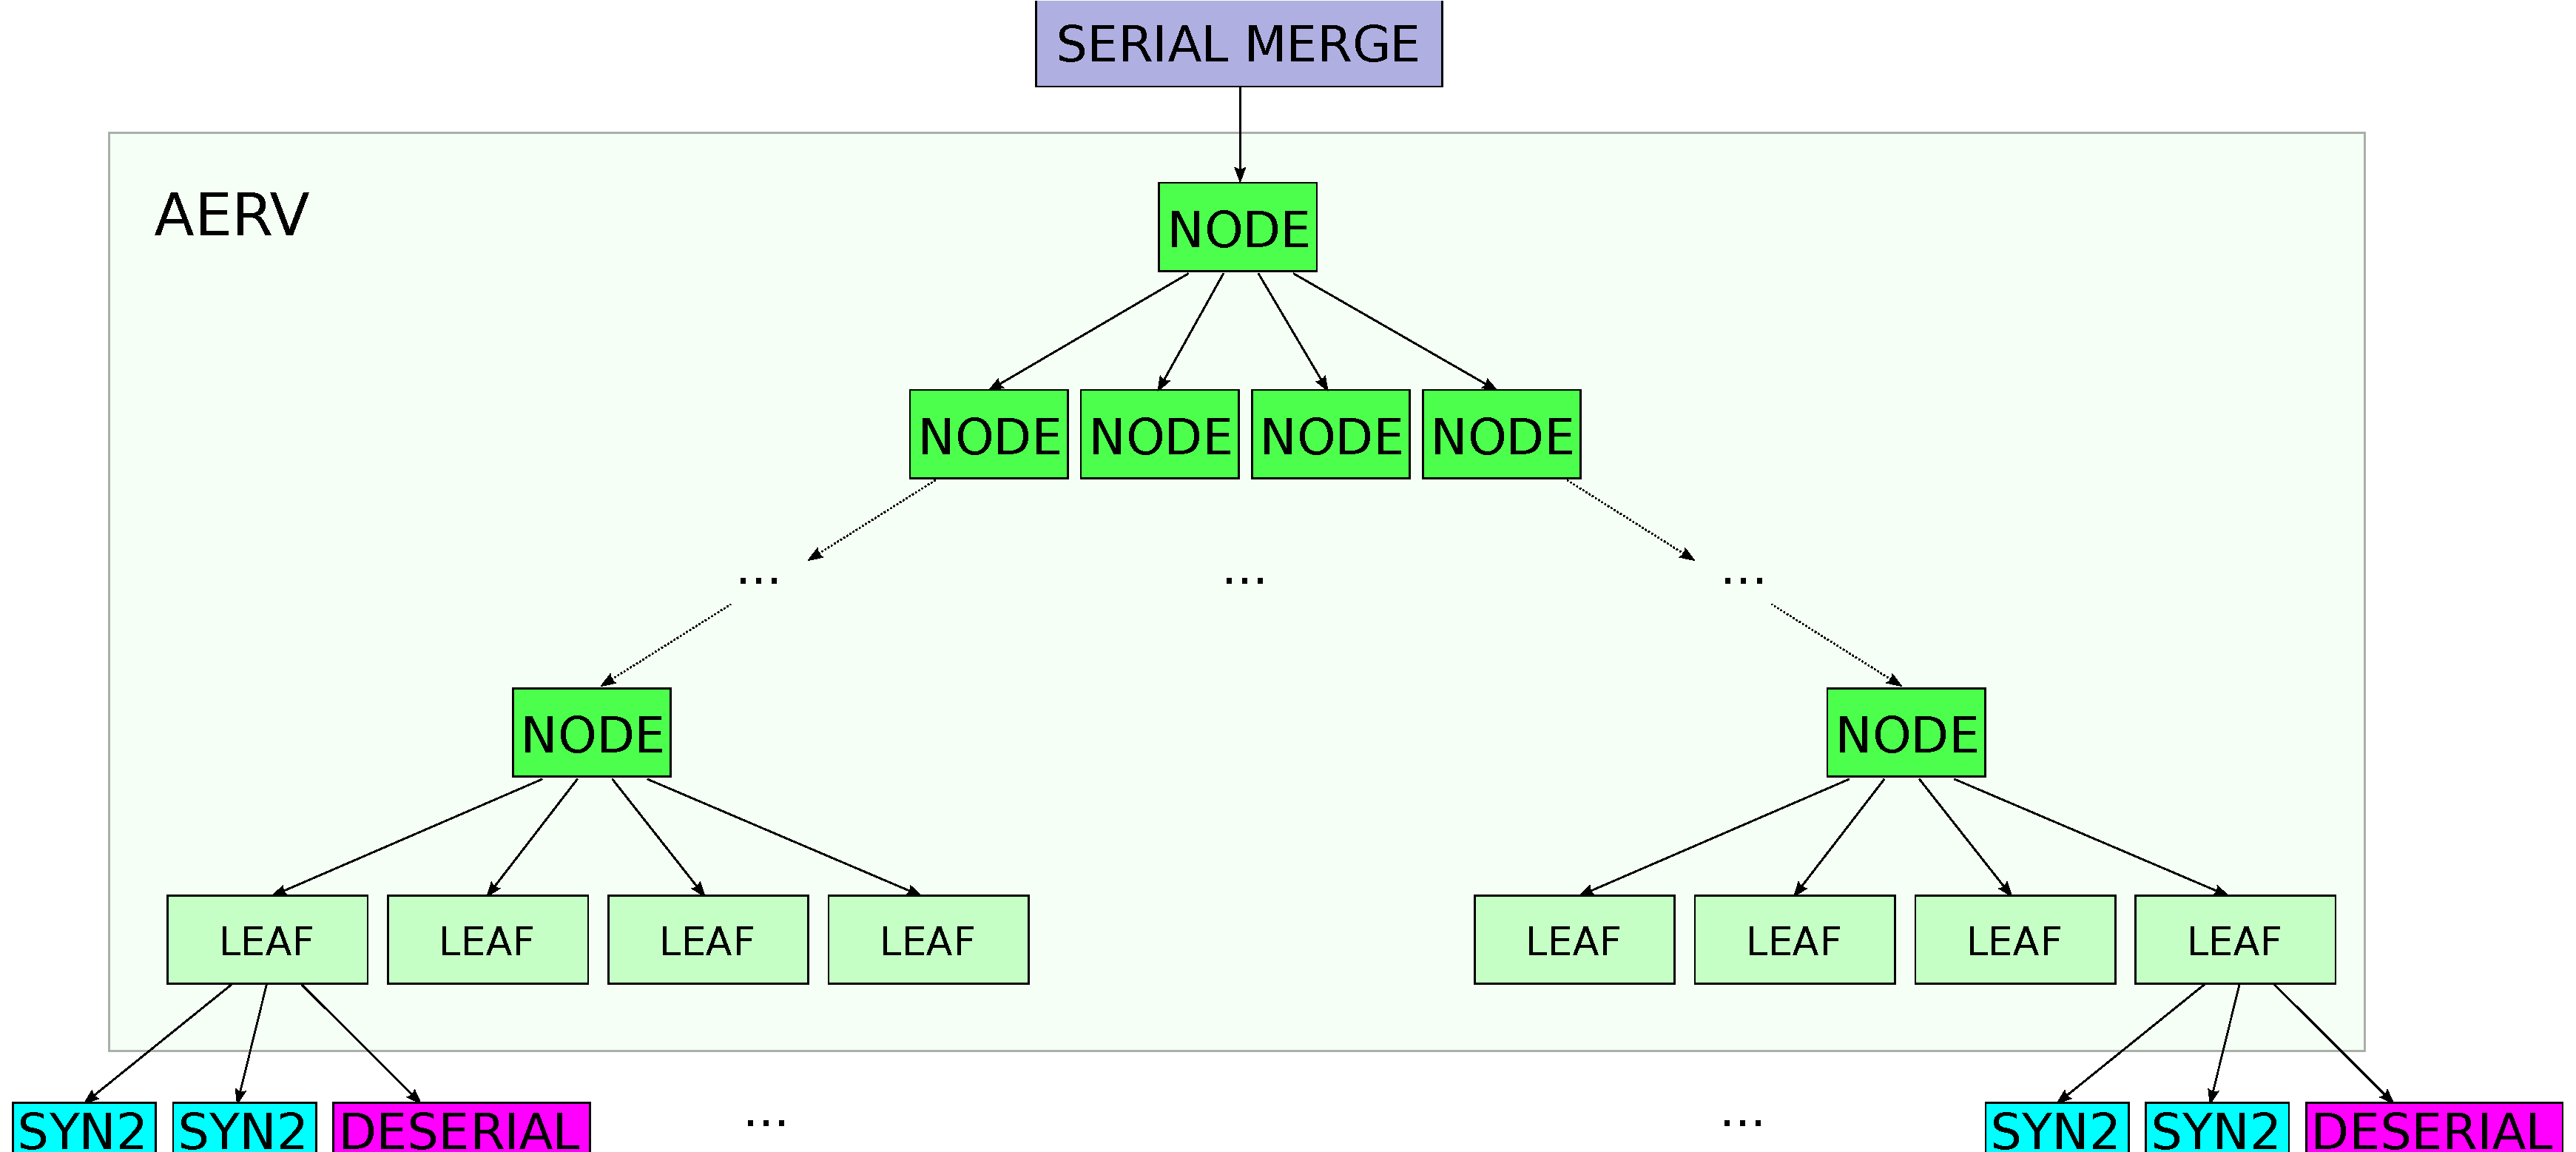
\includegraphics[width=.8\textwidth]{img/aerv.pdf}
\end{center}
Serialized packets from the datapath or router are merged and received at the 
root of the tree.
Datapath packets are destined to a synapse, and router packets
are destined to a memory block through a deserializer. Packets
traverse down the tree. At each node, the head word of the packet is peeled
off to set the direction to forward the rest of the packet.

%%%%%%%%%%%%%%%%%%%%%%%%%%%%%%%%%%%%%%%%%%%%%%%%%%%%%%%%%%%%%%%%%%%%%%%%%%%%%%%
\subsection{AERV NODE \label{sec:AERV_NODE}}

NODE receives packets from its parent and directs their payload to the
child specified by the head word of the packet. Intermediate NODEs 
are configured for 1-of-4 encoding and 4-ary fanout. Leaf NODEs are configured
for 1-of-4 encoding and 3-ary fanout.
The input/output ports are shown as follows:

\begin{center}
  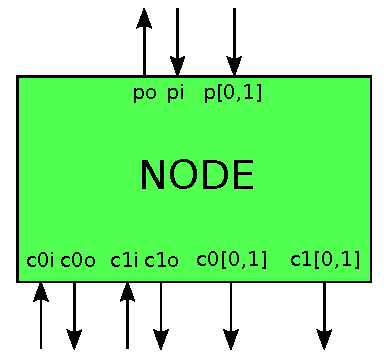
\includegraphics[width=.25\textwidth]{img/aerv_node.pdf}
\end{center}

\subsubsection*{Pseude-code}

\begin{lstlisting}[mathescape]
Repeat {
    Wait for and consume $r$ from the parent.
    Read in a word from the parent
        and use it to set which child to target.
    Send $r$ to the targeted child.
    While (parent is not sending $\neg r$) {
        Relay data from the parent to the targeted child.
    }
    Relay $\neg r$ from the parent to the targeted child.
}
\end{lstlisting}

\subsubsection*{CHP}

\begin{csp}
*[[#{P=r}->P?;[#{P=0}->P?c;C0!r[]#{P=1}->P?c;C1!r]
  [](#{P=0}|#{P=1})&c=0->C0!P?
  [](#{P=0}|#{P=1})&c=1->C1!P?
  []#{P=\neg r}&c=0->C0!P?
  []#{P=\neg r}&c=1->C1!P?
 ]]
\end{csp}

\noindent
To match the CHP to the psuedo-code, we start in the top branch. \\
First, we wait for $r$ and consume it with $P?$. $P?c$ then stores 
the next word in $c$ as the child to target and is followed by $C0!r$ 
or $C1!r$, which send $r$ to the targeted child. 
Note that in the transmitter processes, we simply relay the $r$ from the 
selected child to the parent. Here, we do not know where to send $r$
until receiving the first data word of the packet. \\ 
The second and third branches relay data from the parent to the targeted child. \\
The last two branches relay $\neg r$ to the targeted child. \\

\subsubsection*{HSE}

We implement the HSE

\begin{hse}
*[[pr->pe+;
    [p0->u0+;uu+;pe-;[~p0];v+;c0r+;[c0e];pe+
    []p1->u1+;uu+;pe-;[~p1];v+;c1r+;[c1e];pe+
    ]
  []p0&c0r->c00+;[~c0e];pe-;[~p0];c00-;[c0e];pe+
  []p1&c0r->c01+;[~c0e];pe-;[~p1];c01-;[c0e];pe+
  []p0&c1r->c10+;[~c1e];pe-;[~p0];c10-;[c1e];pe+
  []p1&c1r->c11+;[~c1e];pe-;[~p1];c11-;[c1e];pe+
  []~pr->u0-,u1-;uu-,(c0r-,c1r-;[~c0e&~c1e];pe-),v-
 ]]
\end{hse}

\noindent
To get there, we first directly translate the CHP,

\begin{hse}
*[[pr->pe+;
    [p0->c0+;pe-;[~p0];pe+;c0r+;[c0e]
    []p1->c1+;pe-;[~p1];pe+;c1r+;[c1e]
    ]
  []p0&c0->c00+;[~c0e];pe-;[~p0];c00-;[c0e];pe+
  []p1&c0->c01+;[~c0e];pe-;[~p1];c01-;[c0e];pe+
  []p0&c1->c10+;[~c1e];pe-;[~p0];c10-;[c1e];pe+
  []p1&c1->c11+;[~c1e];pe-;[~p1];c11-;[c1e];pe+
  []~pr&c0->c0r-;[~c0e];c0-;pe-
  []~pr&c1->c1r-;[~c1e];c1-;pe-
 ]]
\end{hse}

\noindent
The top branch in the HSE implements the top branch of the CHP. 2-phase
handshakes implement the $P?$, $C0!r$, and $C1!r$ communications. 
A 4-phase handshake implements $P?c$. The 2-phase handshakes will be 
paired with 2-phase handshakes in the bottom two HSE branches, which
implement the bottom two CHP branches, to return the process to its original
state. \\
The remaining four HSE branches implement the two CHP branches that relay
data from the parent to the selected child.

Since the communications for $\neg r$ reset the process to its
original state, we can combine the last two branches into one.

\begin{hse}
*[[pr->pe+;
    [p0->c0+;pe-;[~p0];pe+;c0r+;[c0e]
    []p1->c1+;pe-;[~p1];pe+;c1r+;[c1e]
    ]
  []p0&c0->c00+;[~c0e];pe-;[~p0];c00-;[c0e];pe+
  []p1&c0->c01+;[~c0e];pe-;[~p1];c01-;[c0e];pe+
  []p0&c1->c10+;[~c1e];pe-;[~p0];c10-;[c1e];pe+
  []p1&c1->c11+;[~c1e];pe-;[~p1];c11-;[c1e];pe+
  []\red{~pr->c0-,c1-;c0r-,c1r-;[~c0e&~c1e];pe-}
 ]]
\end{hse}

\noindent
Next, we overlap the $P?c$ communication with the $C0!r$ and $C1!r$ 
communications and add a reset for $c$ during the $\neg r$ 
communications.

\begin{hse}
*[[pr->pe+;
    [p0->pe-;[~p0];\red{c0+};c0r+;[c0e];\red{pe+}
    []p1->pe-;[~p1];\red{c1+};c1r+;[c1e];\red{pe+}
    ]
  []p0&c0->c00+;[~c0e];pe-;[~p0];c00-;[c0e];pe+
  []p1&c0->c01+;[~c0e];pe-;[~p1];c01-;[c0e];pe+
  []p0&c1->c10+;[~c1e];pe-;[~p0];c10-;[c1e];pe+
  []p1&c1->c11+;[~c1e];pe-;[~p1];c11-;[c1e];pe+
  []~pr->\red{c0-,c1-};c0r-,c1r-;[~c0e&~c1e];pe-
 ]]
\end{hse}

\noindent
$c[0,1]r$ transitions always follow $c[0,1]$ transitions,
respectively, so we can eliminate $c[0,1]$ and use $c[0,1]r$  
in their place.

\begin{hse}
*[[pr->pe+;
    [p0->pe-;[~p0];c0r+;[c0e];pe+
    []p1->pe-;[~p1];c1r+;[c1e];pe+
    ]
  []p0&c0r->c00+;[~c0e];pe-;[~p0];c00-;[c0e];pe+
  []p1&c0r->c01+;[~c0e];pe-;[~p1];c01-;[c0e];pe+
  []p0&c1r->c10+;[~c1e];pe-;[~p0];c10-;[c1e];pe+
  []p1&c1r->c11+;[~c1e];pe-;[~p1];c11-;[c1e];pe+
  []~pr->c0r-,c1r-;[~c0e&~c1e];pe-
 ]]
\end{hse}

\noindent
In the top branch, note that $c[0,1]r$ raise after the parent data clears.
Therefore, we need to introduce state variables $u[0,1]$ to store the first
parent data word.

\begin{hse}
*[[pr->pe+;
    [p0->\red{u0+};pe-;[~p0];c0r+;[c0e];pe+
    []p1->\red{u1+};pe-;[~p1];c1r+;[c1e];pe+
    ]
  []p0&c0r->c00+;[~c0e];pe-;[~p0];c00-;[c0e];pe+
  []p1&c0r->c01+;[~c0e];pe-;[~p1];c01-;[c0e];pe+
  []p0&c1r->c10+;[~c1e];pe-;[~p0];c10-;[c1e];pe+
  []p1&c1r->c11+;[~c1e];pe-;[~p1];c11-;[c1e];pe+
  []~pr->\red{u0-,u1-};c0r-,c1r-;[~c0e&~c1e];pe-
 ]]
\end{hse}

\noindent
We clear the first parent data word before raising $c[0,1]r$ so that the 
subsequent data can be steered to the selected child by simply ANDing the parent 
data with the $c[0,1]r$ lines. If we instead clear the parent data after 
raising one of $c[0,1]r$, we must increase the complexity of the child data 
gates. The cost of storing the first parent data word scales with the data width
whereas the cost of making the child data gates more complicated 
scales with the (data width) $\times$ (number of children). Therefore
storing the first parent data word is cheaper than increasing the complexity
of the child gates. 

Moving on, we introduce state variable $v$ to make the $c[0,1]r$ gates
combinational.

\begin{hse}
*[[pr->pe+;
    [p0->u0+;pe-;[~p0];\red{v+};c0r+;[c0e];pe+
    []p1->u1+;pe-;[~p1];\red{v+};c1r+;[c1e];pe+
    ]
  []p0&c0r->c00+;[~c0e];pe-;[~p0];c00-;[c0e];pe+
  []p1&c0r->c01+;[~c0e];pe-;[~p1];c01-;[c0e];pe+
  []p0&c1r->c10+;[~c1e];pe-;[~p0];c10-;[c1e];pe+
  []p1&c1r->c11+;[~c1e];pe-;[~p1];c11-;[c1e];pe+
  []~pr->u0-,u1-;c0r-,c1r-;[~c0e&~c1e];pe-,\red{v-}
 ]]
\end{hse}

\noindent
Finally, we introduce state variable $uu$ to reduce the number of transistors
in series for the $p_o$ gate.

\begin{hse}
*[[pr->pe+;
    [p0->u0+;\red{uu+};pe-;[~p0];v+;c0r+;[c0e];pe+
    []p1->u1+;\red{uu+};pe-;[~p1];v+;c1r+;[c1e];pe+
    ]
  []p0&c0r->c00+;[~c0e];pe-;[~p0];c00-;[c0e];pe+
  []p1&c0r->c01+;[~c0e];pe-;[~p1];c01-;[c0e];pe+
  []p0&c1r->c10+;[~c1e];pe-;[~p0];c10-;[c1e];pe+
  []p1&c1r->c11+;[~c1e];pe-;[~p1];c11-;[c1e];pe+
  []~pr->u0-,u1-;\red{uu-},(c0r-,c1r-;[~c0e&~c1e];pe-),v-
 ]]
\end{hse}

\noindent
which completes our expansion.

\subsubsection*{PRS}

\begin{prs2}
u0 | u1 -> uu+
~u0 & ~u1 -> uu-
\end{prs2}

\begin{prs2}
pr & ~uu | c0e | c1e -> pe+
(~pr | uu) & ~c0e & ~c1e -> pe-
\end{prs2}

\begin{prs2}
p0 & ~v -> u0+
~pr -> u0-

p1 & ~v -> u1+
~pr -> u1-
\end{prs2}

\begin{prs2}
uu & ~p0 & ~p1 -> v+
~uu -> v-
\end{prs2}

\begin{prs2}
v & u0 -> c0r+
~v | ~u0 -> c0r-

v & u1 -> c1r+
~v | ~u1 -> c1r-
\end{prs2}

\begin{prs2}
p0 & c0r -> c00+
~p0 | ~c0r -> c00-

p1 & c0r -> c01+
~p1 | ~c0r -> c01-

p0 & c1r -> c10+
~p0 | ~c1r -> c10-

p1 & c1r -> c11+
~p1 | ~c1r -> c11-
\end{prs2}

\noindent
4-ary fanout, 1-of-4 encoding approximate accounting:

\begin{center}
    \begin{tabular}{|r|l|l|}
    \hline
    rule & transistor count & comments \\ \hline
    $uu$ & 8 & \\ \hline
    $p_o$ & 12 & \\ \hline
    $u[0,1,2,3]$ & 28 & \\ \hline
    $v$ & 10 & \\ \hline
    $c[0,1,2,3]r$ & 16 & \\ \hline
    $c[0,1,2,3][0,1,2,3]$ & 64 & \\ \hline
    \hline total & 138 & \\ \hline
    \end{tabular}
\end{center}

\noindent
3-ary fanout, 1-of-4 encoding approximate accounting:

\begin{center}
    \begin{tabular}{|r|l|l|}
    \hline
    rule & transistor count & comments \\ \hline
    $uu$ & 6 & \\ \hline
    $p_o$ & 10 & \\ \hline
    $u[0,1,2]$ & 21 & \\ \hline
    $v$ & 10 & \\ \hline
    $c[0,1,2]r$ & 12 & \\ \hline
    $c[0,1,2][0,1,2,3]$ & 48 & \\ \hline
    \hline total & 107 & \\ \hline
    \end{tabular}
\end{center}

\subsubsection*{CMOS-implementable PRS}

\begin{prs2}
~u0 -> _u0+
u0 -> _u0-

~u1 -> _u1+
u1 -> _u1-
\end{prs2}

\begin{prs2}
~_u0 | ~_u1 -> uu+
_u0 & _u1 -> uu-
\end{prs2}

\begin{prs2}
~_pr & ~uu | ~_c0e | ~_c1e -> pe+
(_pr | uu) & _c0e & _c1e -> pe-
\end{prs2}

\begin{prs2}
~_v -> __v+
_v -> __v-
\end{prs2}

\begin{prs2}
~p0 -> _p0+
p0 -> _p0-

~p1 -> _p1+
p1 -> _p1-
\end{prs2}

\begin{prs2}
~_p0 & ~__v -> u0+
_pr -> u0-

~_p1 & ~__v -> u1+
_pr -> u1-
\end{prs2}

\begin{prs2}
uu & _p0 & _p1 -> _v-
~uu -> _v+
\end{prs2}

\begin{prs2}
__v & u0 -> _c0r-
~__v | ~u0 -> _c0r+

__v & u1 -> _c1r-
~__v | ~u1 -> _c1r+
\end{prs2}

\begin{prs2}
~_p0 & ~_c0r -> c00+
_p0 | _c0r -> c00-

~_p1 & ~_c0r -> c01+
_p1 | _c0r -> c01-

~_p0 & ~_c1r -> c10+
_p0 | _c1r -> c10-

~_p1 & ~_c1r -> c11+
_p1 | _c1r -> c11-
\end{prs2}

\begin{prs2}
~pe -> _pe+
pe -> _pe-
\end{prs2}

\noindent
4-ary fanout, 1-of-4 encoding accounting:

\begin{center}
    \begin{tabular}{|r|l|l|}
    \hline
    rule & transistor count & comments \\ \hline
    $\_u[0,1,2,3]$ & 8 & \\ \hline
    $uu$ & 8 & \\ \hline
    $p_o$ & 12 & \\ \hline
    $\_\_v$ & 2 & \\ \hline
    $\_p[0,1,2,3]$ & 8 \\ \hline
    $u[0,1,2,3]$ & 28 & \\ \hline
    $\_v$ & 10 & \\ \hline
    $\_c[0,1,2,3]r$ & 16 & \\ \hline
    $c[0,1,2,3][0,1,2,3]$ & 64 & \\ \hline
    \hline total & 156 & \\ \hline
    \end{tabular}
\end{center}

\noindent
3-ary fanout, 1-of-4 encoding accounting:

\begin{center}
    \begin{tabular}{|r|l|l|}
    \hline
    rule & transistor count & comments \\ \hline
    $\_u[0,1,2]$ & 6 & \\ \hline
    $uu$ & 6 & \\ \hline
    $p_o$ & 10 & \\ \hline
    $\_\_v$ & 2 & \\ \hline
    $\_p[0,1,2,3]$ & 8 \\ \hline
    $u[0,1,2]$ & 21 & \\ \hline
    $\_v$ & 10 & \\ \hline
    $\_c[0,1,2]r$ & 12 & \\ \hline
    $c[0,1,2][0,1,2,3]$ & 48 & \\ \hline
    \hline total & 123 & \\ \hline
    \end{tabular}
\end{center}

%%%%%%%%%%%%%%%%%%%%%%%%%%%%%%%%%%%%%%%%%%%%%%%%%%%%%%%%%%%%%%%%%%%%%%%%%%%%%%%
\subsection{AERV LEAF \label{sec:AERV_LEAF}}

We designed a custom leaf because the synapse needed buffering.

\subsubsection*{HSE}

\begin{hse}
*[[pr->pe+;
    [p0->u0+;uu+;pe-;[~p0];v+;c0r+;pe+
    []p1->u1+;uu+;pe-;[~p1];v+;c1r+;pe+
    []p2->u2+;uu+;pe-;[~p2];v+;c2r+;[c2i];pe+
    ]
  []p0&c0r->[c00e];c000+;pe-;[~c00e&~p0];c000-;pe+;
  []p1&c0r->[c00e];c001+;pe-;[~c00e&~p1];c001-;pe+;
  []p2&c0r->[c01e];c010+;pe-;[~c01e&~p2];c010-;pe+;
  []p3&c0r->[c01e];c011+;pe-;[~c01e&~p3];c011-;pe+;
  []p0&c1r->[c10e];c100+;pe-;[~c10e&~p0];c100-;pe+;
  []p1&c1r->[c10e];c101+;pe-;[~c10e&~p1];c101-;pe+;
  []p2&c1r->[c11e];c100+;pe-;[~c11e&~p2];c110-;pe+;
  []p3&c1r->[c11e];c101+;pe-;[~c11e&~p3];c111-;pe+;
  []p0&c2r->;c20+;[~c2i];pe-;[~p0];c20-;[c2i];pe+;
  []p1&c2r->;c21+;[~c2i];pe-;[~p1];c21-;[c2i];pe+;
  []p2&c2r->;c22+;[~c2i];pe-;[~p2];c22-;[c2i];pe+;
  []p3&c2r->;c23+;[~c2i];pe-;[~p3];c23-;[c2i];pe+;
  []~pr&c0r->u0-;(uu-;v-),(c0r-;pe-)
  []~pr&c1r->u1-;(uu-;v-),(c1r-;pe-)
  []~pr&c2r->u2-;(uu-;v-),(c2r-;[~c2i];pe-)
 ]]
\end{hse}

\subsubsection*{PRS}

\begin{prs2}
u0 | u1 | u2 -> uu+
~u0 & ~u1 & ~u2 -> uu-
\end{prs2}

\begin{prs2}
pp & ~uu | c0r & ~c0[0,1][0,1] | c1r & ~c1[0,1][0,1] | c2i -> pe+
(~pp | uu) & (~c0r | c0[0,1][0,1]) & (~c1r | c1[0,1][0,1]) & ~c2i -> pe-
\end{prs2}

\begin{prs2}
p[0,1,2] & ~v -> u[0,1,2]+
~pr -> u[0,1,2]-
\end{prs2}

\begin{prs2}
uu & ~p[0,1,2] -> v+
~uu -> v-
\end{prs2}

\begin{prs2}
v & u[0,1,2] -> c[0,1,2]r+
~v | ~u[0,1,2] -> c[0,1,2]r-
\end{prs2}

\begin{prs2}
p0 & c[0,1]r & c[0,1]0e -> c[0,1]00+
~p0 & ~c[0,1]0e -> c[0,1]00-

p1 & c[0,1]r & c[0,1]0e -> c[0,1]01+
~p1 & ~c[0,1]0e -> c[0,1]01-

p2 & c[0,1]r & c[0,1]0e -> c[0,1]10+
~p2 & ~c[0,1]0e -> c[0,1]10-

p3 & c[0,1]r & c[0,1]1e -> c[0,1]11+
~p3 & ~c[0,1]1e -> c[0,1]11-
\end{prs2}

\begin{prs2}
p[0,1,2,3] & c2r -> c2[0,1,2,3]+
~p[0,1,2,3] | ~c2r -> c2[0,1,2,3]-
\end{prs2}

\noindent
approximate accounting:

\begin{center}
    \begin{tabular}{|r|l|l|}
    \hline
    rule & transistor count & comments \\ \hline
    $uu$ & 6 & \\ \hline
    $p_o$ & 26 & \\ \hline
    $u[0,1,2]$ & 21 & \\ \hline
    $v$ & 9 & \\ \hline
    $c[0,1,2]r$ & 12 & \\ \hline
    $c[0,1][0,1][0,1]$ & 72 & \\ \hline
    $c2[0,1,2,3]$ & 16 & \\
    \hline total & 162 & \\ \hline
    \end{tabular}
\end{center}

\subsubsection*{CMOS-implementable PRS}

\begin{prs2}
~__u0 | ~_u1 | ~_u2 -> uu+
_u0 & _u1 & _u2 -> uu-
\end{prs2}

\begin{prs2}
~uu -> _uu+
uu -> _uu-
\end{prs2}

\begin{prs2}
pr & _uu | c0r & _c0[0,1][0,1] | c1r & _c1[0,1][0,1] | c2i -> _pe-
(~pr | ~_uu) & (~c0r | ~_c0[0,1][0,1]) & (~c1r | ~_c1[0,1][0,1]) & ~c2i -> _pe+
\end{prs2}

\begin{prs2}
~v -> _v+
v -> _v-
\end{prs2}

\begin{prs2}
p[0,1,2] & _v -> _u[0,1,2]-
~pr -> _u[0,1,2]+
\end{prs2}

\begin{prs2}
~_uu & ~p[0,1,2] -> v+
_uu -> v-
\end{prs2}

\begin{prs2}
~_v & ~_u[0,1,2] -> c[0,1,2]r+
_v | _u[0,1,2] -> c[0,1,2]r-
\end{prs2}

\begin{prs2}
p0 & c[0,1]r & c[0,1]0e -> _c[0,1]00-
~p0 & ~c[0,1]0e -> _c[0,1]00+

p1 & c[0,1]r & c[0,1]0e -> _c[0,1]01-
~p1 & ~c[0,1]0e -> _c[0,1]01+

p2 & c[0,1]r & c[0,1]0e -> _c[0,1]10-
~p2 & ~c[0,1]0e -> _c[0,1]10+

p3 & c[0,1]r & c[0,1]1e -> _c[0,1]11-
~p3 & ~c[0,1]1e -> _c[0,1]11+
\end{prs2}

\begin{prs2}
p[0,1,2,3] & c2r -> _c2[0,1,2,3]-
~p[0,1,2,3] | ~c2r -> _c2[0,1,2,3]+
\end{prs2}

% interface inverters

\begin{prs2}
~_pr -> pr+
_pr -> pr-
\end{prs2}

\begin{prs2}
~_c[0,1]00 -> __c[0,1]00+
_c[0,1]00 -> __c[0,1]00-

~_c[0,1]01 -> __c[0,1]01+
_c[0,1]01 -> __c[0,1]01-

~_c[0,1]10 -> __c[0,1]10+
_c[0,1]10 -> __c[0,1]10-

~_c[0,1]11 -> __c[0,1]11+
_c[0,1]11 -> __c[0,1]11-
\end{prs2}

\begin{prs2}
~_c2[0,1,2,3] -> __c2[0,1,2,3]+
_c2[0,1,2,3] -> __c2[0,1,2,3]-
\end{prs2}

\noindent
accounting:

\begin{center}
    \begin{tabular}{|r|l|l|}
    \hline
    rule & transistor count & comments \\ \hline
    $uu$ & 6 & \\ \hline
    $\_uu$ & 2 & \\ \hline
    $\_p_o$ & 26 & \\ \hline
    $\_v$ & 2 & \\ \hline
    $\_u[0,1,2]$ & 21 & \\ \hline
    $v$ & 9 & \\ \hline
    $c[0,1,2]r$ & 12 & \\ \hline
    $\_c[0,1][0,1][0,1]$ & 40 & staticized by $\_\_c[0,1][0,1][0,1]$ \\ \hline
    $\_c2[0,1,2,3]$ & 16 & \\
    $pr$ & 2 & \\
    $\_c[0,1][0,1][0,1]$ & 32 & staticizes $\_c[0,1][0,1][0,1]$ \\ \hline
    $\_\_c2[0,1,2,3]$ & 8 & \\ \hline
    \hline total & 176 & \\ \hline
    \end{tabular}
\end{center}

%%%%%%%%%%%%%%%%%%%%%%%%%%%%%%%%%%%%%%%%%%%%%%%%%%%%%%%%%%%%%%%%%%%%%%%%%%%%%%%
\subsection{AERV MERGE ACK \label{sec:AERV_MERGE_ACK}}

The MERGE ACK process merges the $r$ communications at the receiver leaves
with the acknowledges from the synapses or deserializer.

\subsubsection*{HSE}

\begin{hse}
*[[pr&~c0e&~ci1->pe+;
  []pr&c0e->c+;pe-;[~c0e];c-;pe+
  []pr&c1e->c+;pe-;[~c1e];c-;pe+
  []~pr->pe-
 ]]
\end{hse}

\subsubsection*{PRS}

\begin{prs}
pr & ~c0e -> pe+
~pr | c0i -> pe-
\end{prs}

\subsubsection*{CMOS-implementable PRS}

\begin{prs2}
~pr -> _pr+
pr -> _pr-
\end{prs2}

\begin{prs2}
~_pr & ~c0i -> pe+
_pr | c0i -> pe-
\end{prs2}

\noindent
accounting:

\begin{center}
    \begin{tabular}{|r|l|l|}
    \hline
    rule & transistor count & comments \\ \hline
    $\_pr$ & 2 & \\ \hline
    $\_po$ & 4 & \\ \hline
    \hline total & 6 & \\ \hline
    \end{tabular}
\end{center}

%%%%%%%%%%%%%%%%%%%%%%%%%%%%%%%%%%%%%%%%%%%%%%%%%%%%%%%%%%%%%%%%%%%%%%%%%%%%%%%
\subsection{AERV HALF BUF \label{sec:AERV_HALF_BUF}}

The HALF BUF is a WCHB and provides half a cycle of slack between the receiver
and the synapse. 

\begin{hse}
*[xe+;[X&ye];Y+;xe-;[~X&~ye];Y-]
\end{hse}

\begin{prs}
~y0 & ~y1 -> xe+
y0 | y1 -> xe-
\end{prs}

\begin{prs2}
x0 & ye -> y0+
~x0 & ~ye -> y0-

x1 & ye -> y1+
~x1 & ~ye -> y1-
\end{prs2}

\subsubsection*{CMOS-implementable PRS}

\begin{prs2}
~_y0 -> __y0+
_y0 -> __y0-

~_y1 -> __y1+
_y1 -> __y1-
\end{prs2}

\begin{prs2}
~__y0 & ~__y1 -> xe+
__y0 | __y1 -> xe-
\end{prs2}

\begin{prs2}
x0 & ye -> _y0-
~x0 & ~ye -> _y0+

x1 & ye -> _y1-
~x1 & ~ye -> _y1+
\end{prs2}

\noindent
Accounting:

\begin{center}
    \begin{tabular}{|r|l|l|}
    \hline
    rule & transistor count & comments \\ \hline
    $\_\_y[0,1]$ & 8 & staticizes $\_y[0,1]$ \\ \hline
    $\_y[0,1]$ & 8 & staticized by $\_\_y[0,1]$ \\ \hline
    $\_x_e$ & 4 & \\ \hline
    \hline total & 20 & \\ \hline
    \end{tabular}
\end{center}

%%%%%%%%%%%%%%%%%%%%%%%%%%%%%%%%%%%%%%%%%%%%%%%%%%%%%%%%%%%%%%%%%%%%%%%%%%%%%%%
\section{Interfaces}

We need interfaces to covert between the serial data format used within the transmitter
and receiver and the standard, parallel data formate used by environment.

%%%%%%%%%%%%%%%%%%%%%%%%%%%%%%%%%%%%%%%%%%%%%%%%%%%%%%%%%%%%%%%%%%%%%%%%%%%%%%%
\subsection{Deserializer \label{sec:DESERIAL}}

The deserializer converts 1ofN serial data into Mx1ofN parallel data.
As previously seen in Figure~\ref{fig:aer_system}, we place a deserializer 
between the transmitter and the datapath circuitry. We also place deserializers
between the receiver and the neuron configuration memory blocks.

\begin{center}
  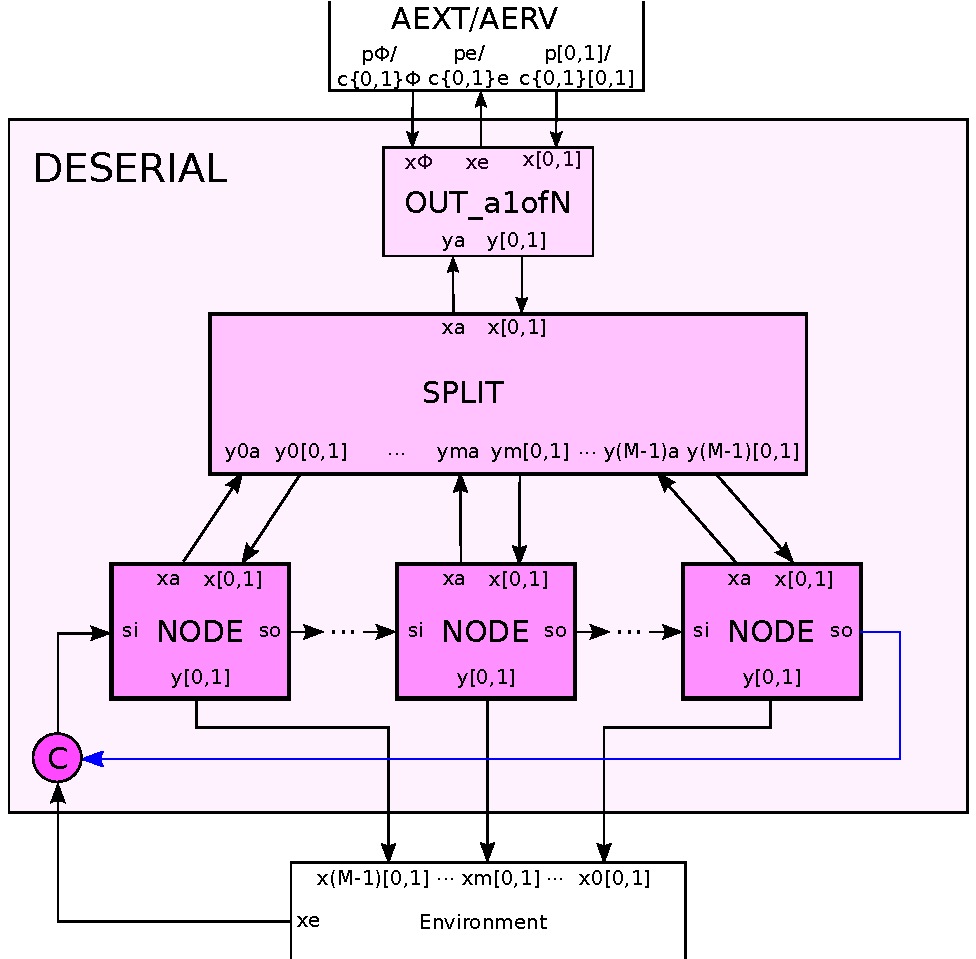
\includegraphics[width=.45\textwidth]{img/deserial.pdf}
\end{center}

An OUT a1ofN process converts the AEXT/AERV serial communication protocol to the
standard a1ofN protocol. A ring of NODES receives data from a central SPLIT
process and sequence the serial words into their respective place in the parallel 
output. 

%%%%%%%%%%%%%%%%%%%%%%%%%%%%%%%%%%%%%%%%%%%%%%%%%%%%%%%%%%%%%%%%%%%%%%%%%%%%%%%
\subsubsection{DESERIAL OUT a1ofN \label{sec:OUT_a1ofN}}

This process converts the transmitter and receiver serial format to a1ofN channel.

\subsubsection*{HSE}

\begin{hse}
*[[xr];xe+;[~xr];xe-]

*[[x0->y0+;[ya];xe-;[~x0];y0-;[~ya];xe+
  []x1->y1+;[ya];xe-;[~x1];y1-;[~ya];xe+
 ]]
\end{hse}

\subsubsection*{PRS}

\begin{prs2}
xr & ~ya -> xe+
~xr | ya -> xe-
\end{prs2}

\begin{prs2}
x0 -> y0+
~x0 -> y0-

x1 -> y1+
~x1 -> y1-
\end{prs2}

\subsubsection*{CMOS-implementable PRS}

\begin{prs2}
~xr -> _xr+
xr -> _xr-
\end{prs2}

\begin{prs2}
~_xr & ~ya -> xe+
_xr | ya -> xe-
\end{prs2}

\begin{prs2}
x0 -> y0+
~x0 -> y0-

x1 -> y1+
~x1 -> y1-
\end{prs2}

\noindent
1-of-4 accounting:

\begin{center}
    \begin{tabular}{|r|l|l|}
    \hline
    rule & transistor count & comments \\ \hline
    $\_xr$ & 2 & \\ \hline
    $x_e$ & 4 & \\ \hline
    $\_y[0,1,2,3]$ & 0 & wires \\ \hline
    \hline total & 6 & \\ \hline
    \end{tabular}
\end{center}

%%%%%%%%%%%%%%%%%%%%%%%%%%%%%%%%%%%%%%%%%%%%%%%%%%%%%%%%%%%%%%%%%%%%%%%%%%%%%%%
\subsubsection{DESERIAL SPLIT \label{sec:DESERIAL_SPLIT}}

SPLIT takes incoming words and routes them to their respective locations
in the parallel output.

\subsubsection*{HSE}

\noindent
For $M$ words per packet,

\begin{hse}
*[[x0->y00+,..,y(M\-1)0+;[y0a|..|y(M\-1)a];xa+;
    [~x0];y00-,..,y(M\-1)1-;[~y0a&..&~y(M\-1)a];xa-
  []x1->y01+,..,y(M\-1)1+;[y0a|..|y(M\-1)a];xa+;
    [~x0];y01-,..,y(M\-1)1-;[~y0a&..&~y(M\-1)a];xa-
 ]]
\end{hse}

\noindent
For a 2-word packet,

\begin{hse}
*[[x0->y00+,y10+;[y0a|y1a];xa+;
    [~x0];y00-,y01-;[~y0a&~y1a];xa-
  []x1->y01+,y11+;[y0a|y1a];xa+;
    [~x0];y01-,y11-;[~y0a&~y1a];xa-
 ]]
\end{hse}

\subsubsection*{PRS}

\begin{prs2}
x0 -> y00+, y10+
~x0 -> y00-, y10-

x1 -> y01+, y11+
~x1 -> y01-, y11-
\end{prs2}

\begin{prs2}
y0a | y1a -> xa+
~y0a & ~y1a -> xa-
\end{prs2}

\noindent
1-of-4 approximate scaling:

\begin{center}
    \begin{tabular}{|r|l|l|}
    \hline
    rule & transistor count & comments \\ \hline
    $y[0..M-1][0,1,2,3]$ & 0 & wires \\ \hline
    $xa$ & $8(M-1)/3$ & 4-ary OR-tree approx. \\ \hline
    \hline approx. total & $3M-2$ & \\ \hline
    \end{tabular}
\end{center}

\subsubsection*{CMOS-implementable PRS}

\begin{prs2}
x0 -> _y00-, _y10-
~x0 -> _y00+, _y10+

x1 -> _y01-, _y11-
~x1 -> _y01+, _y11+
\end{prs2}

\begin{prs2}
~_y0a | ~_y1a -> xa+
_y0a & _y1a -> xa-
\end{prs2}

\noindent
1-of-4 accounting:

\begin{center}
    \begin{tabular}{|r|l|l|}
    \hline
    rule & transistor count & comments \\ \hline
    \hline \multicolumn{3}{|l|}{M=4} \\ \hline
    $y[0..3][0,1,2,3]$ & 8 & \\ \hline
    $xa$ & 8 & \\ \hline
    total & 16 & \\ \hline
    \hline \multicolumn{3}{|l|}{M=6} \\ \hline
    $y[0..5][0,1,2,3]$ & 8 & \\ \hline
    $xa$ & 18 & \\ \hline
    total & 26 & \\ \hline
    \end{tabular}
\end{center}

%%%%%%%%%%%%%%%%%%%%%%%%%%%%%%%%%%%%%%%%%%%%%%%%%%%%%%%%%%%%%%%%%%%%%%%%%%%%%%%
\subsubsection{DESERIAL NODE \label{sec:DESERIAL_NODE}}

NODE latches data from SPLIT.

\subsubsection*{HSE}

\begin{hse}
*[[si];
  [x0->y0+;xa+;[~x0];s+;so+;xa-;[~si];y0-;s-;so-
  []x1->y1+;xa+;[~x1];s+;so+;xa-;[~si];y1-;s-;so-
  ]
 ]
\end{hse}

The $s$ state variable is necessary for bubble reshuffling. 

\subsubsection*{PRS}

\begin{prs2}
~s & si & x0 -> y0+
~si -> y0-

~s & si & x1 -> y1+
~si -> y1-
\end{prs2}

\begin{prs2}
~so & vy -> xa+
so | ~vy -> xa-
\end{prs2}

\begin{prs2}
vy & ~x0 & ~x1 -> s+
~vy -> s-
\end{prs2}

\begin{prs2}
s -> so+
~s -> so-
\end{prs2}

\begin{prs2}
y0 | y1 -> vy+
~y0 & ~y1 -> vy-
\end{prs2}

\noindent
1-of-4 approximate accounting:

\begin{center}
    \begin{tabular}{|r|l|l|}
    \hline
    rule & transistor count & comments \\ \hline
    $y[0,1,2,3]$ & 32 & \\ \hline
    $xa$ & 4 & \\ \hline
    $s$ & 6 & staticized by $s_o$ \\ \hline
    $s_o$ & 4 & staticizes $s$ \\ \hline
    $vy$ & 8 & \\ \hline
    \hline total & 54 & \\ \hline
    \end{tabular}
\end{center}

\subsubsection*{CMOS-implementable PRS}

\begin{prs2}
~_s -> __s+
_s -> __s-
\end{prs2}

\begin{prs2}
~__s & ~_si & ~_x0 -> y0+
_si -> y0-

~__s & ~_si & ~_x1 -> y1+
_si -> y1-
\end{prs2}

\begin{prs2}
_so & vy -> _xa-
~_so | ~vy -> _xa+
\end{prs2}

\begin{prs2}
vy & _x0 & _x1 -> _s-
~vy -> _s+
\end{prs2}

\begin{prs2}
__s -> _so-
~__s -> _so+
\end{prs2}

\begin{prs2}
~y0 -> _y0+
y0 -> _y0-

~y1 -> _y1+
y1 -> _y1-
\end{prs2}

\begin{prs2}
~_y0 | ~_y1 -> vy+
_y0 & _y1 -> vy-
\end{prs2}

\noindent
1-of-4 accounting:

\begin{center}
    \begin{tabular}{|r|l|l|}
    \hline
    rule & transistor count & comments \\ \hline
    $\_\_s$ & 4 & staticizes $s$ \\ \hline
    $y[0,1,2,3]$ & 16 & staticized by $\_y[0,1,2,3]$ \\ \hline
    $\_xa$ & 4 & \\ \hline
    $\_s$ & 4 & staticized by $\_\_s$ \\ \hline
    $\_so$ & 2 & \\ \hline
    $\_y[0,1,2,3]$ & 16 & staticizes $y[0,1,2,3]$ \\ \hline
    $vy$ & 8 & \\ \hline
    \hline total & 54 & \\ \hline
    \end{tabular}
\end{center}

%%%%%%%%%%%%%%%%%%%%%%%%%%%%%%%%%%%%%%%%%%%%%%%%%%%%%%%%%%%%%%%%%%%%%%%%%%%%%%%
\subsubsection{DESERIAL C \label{sec:DESERIAL_C}}

C in the deserializer is a C-element taking in the environment enable signal 
and the last node's $s_o$ signal to produce first node's $s_i$ signal. 
$s_i$ indicates whether we are in the up or down phase of the serial-to-parallel conversion.

\subsubsection*{PRS}

\begin{prs2}
~so & xe -> si+
so & ~xe -> si-
\end{prs2}

\subsubsection*{CMOS-implementable PRS}

\begin{prs2}
_so & xe -> _si-
~_so & ~xe -> _si+
\end{prs2}

\noindent
A C-element costs 8 transistors.

%%%%%%%%%%%%%%%%%%%%%%%%%%%%%%%%%%%%%%%%%%%%%%%%%%%%%%%%%%%%%%%%%%%%%%%%%%%%%%%
\subsubsection{Accounting}

The cost of the deserializer depends on the length of the packet. We first 
consider the approximate scaling.

\begin{center}
    \begin{tabular}{|r|l|l|l|}
    \hline
    component & transistors/component & components/deserializer & transistors/deserializer \\ \hline
    OUT a1ofN & 6 & 1 & 6 \\ \hline
    SPLIT & $3M-2$ & 1 & $3M-2$ \\ \hline
    NODE & 54 & $M$ & $54M$ \\ \hline
    C & 8 & 1 & 8 \\ \hline
    \hline \multicolumn{3}{|r|}{approx. transistors/deserializer} & $57M+12$ \\ \hline
    \end{tabular}
\end{center}

\noindent
To deserialize the transmitter packets, we need 6 NODEs.

\begin{center}
    \begin{tabular}{|r|l|l|l|}
    \hline
    component & transistors/component & components/deserializer & transistors/deserializer \\ \hline
    OUT a1ofN & 6 & 1 & 6 \\ \hline
    SPLIT & 26 & 1 & 26 \\ \hline
    NODE & 54 & 6 & 324 \\ \hline
    C & 8 & 1 & 8 \\ \hline
    \hline \multicolumn{3}{|r|}{total transistors/deserializer} & 364 \\ \hline
    \end{tabular}
\end{center}

\noindent
To deserialize the memory packets, we need 4 NODEs.

\begin{center}
    \begin{tabular}{|r|l|l|l|}
    \hline
    component & transistors/component & components/deserializer & transistors/deserializer \\ \hline
    OUT a1ofN & 6 & 1 & 6 \\ \hline
    SPLIT & 16 & 1 & 16 \\ \hline
    NODE & 54 & 4 & 216 \\ \hline
    C & 8 & 1 & 8 \\ \hline
    \hline \multicolumn{3}{|r|}{total transistors/deserializer} & 246 \\ \hline
    \end{tabular}
\end{center}

%%%%%%%%%%%%%%%%%%%%%%%%%%%%%%%%%%%%%%%%%%%%%%%%%%%%%%%%%%%%%%%%%%%%%%%%%%%%%%%
\subsection{Serializer \label{sec:SERIAL}}

The serializer converts Mx1ofN data into in 1ofN serial data.
We cannot use an a1ofN-to-serial converter like we could with the deserializer
because the serial protocol requires a signal indicating the end of a packet.

This design uses a ring of NODES to sequence the words of an eMx1ofN 
channel. A SEQ process ensures the proper sequencing of the serial protocol.

\begin{center}
  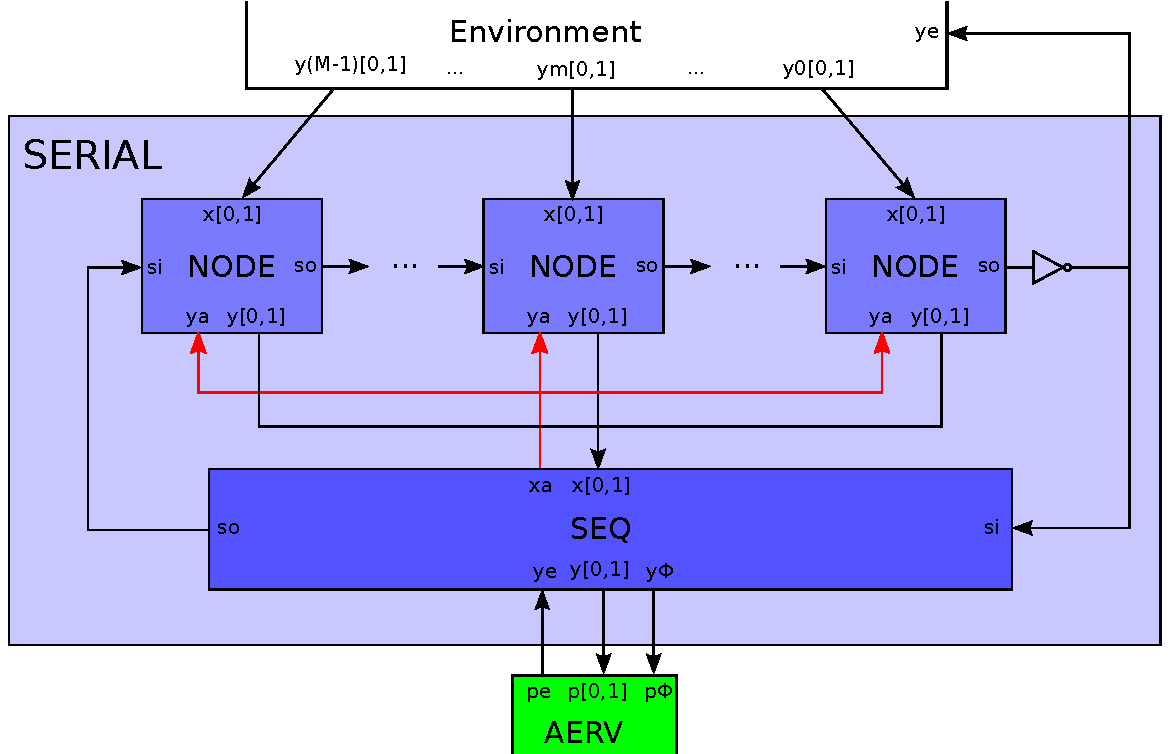
\includegraphics[width=.7\textwidth]{img/serial.pdf}
\end{center}

Note the shared $ya$ and $y[0,1]$ between the NODE processes.

%%%%%%%%%%%%%%%%%%%%%%%%%%%%%%%%%%%%%%%%%%%%%%%%%%%%%%%%%%%%%%%%%%%%%%%%%%%%%%%
\subsubsection{SERIAL NODE \label{sec:SERIAL_NODE}}

\subsubsection*{HSE}

\begin{hse}
*[[si];
  [x0->y0+;[ya];u+;y0-;[~ya];so+;[~si];u-;[~x0];so-
  []x1->y1+;[ya];u+;y1-;[~ya];so+;[~si];u-;[~x1];so-
 ]]
\end{hse}

\subsubsection*{PRS}

\begin{prs2}
x0 & ~u & si -> y0+
u & ~so -> y0-

x1 & ~u & si -> y1+
u & ~so -> y1-
\end{prs2}

\begin{prs2}
si & ya -> u+
~si -> u-
\end{prs2}

\begin{prs2}
u & ~ya -> so+
~u & ~x0 & ~x1 -> so-
\end{prs2}

\subsubsection*{CMOS-implementable PRS}

\begin{prs2}
~_u -> __u+
_u -> __u-
\end{prs2}

\begin{prs2}
~so -> _so+
so -> _so-
\end{prs2}

\begin{prs2}
~_x0 & ~__u & ~_si -> y0+
__u & _so -> y0-

~_x1 & ~__u & ~_si -> y1+
__u & _so -> y1-
\end{prs2}

\begin{prs2}
~_si -> __si+
_si -> __si-
\end{prs2}

\begin{prs2}
__si & ya -> _u-
~__si -> _u+
\end{prs2}

\begin{prs2}
~__u -> ___u+
__u -> ___u-
\end{prs2}

\begin{prs2}
~___u & ~ya -> so+
___u & _x0 & _x1 -> so-
\end{prs2}

\begin{prs2}
~y0 -> _y0+
y0 -> _y0-

~y1 -> _y1+
y1 -> _y1-
\end{prs2}

\noindent
1-of-4 accounting:

\begin{center}
    \begin{tabular}{|r|l|l|}
    \hline
    rule & transistor count & comments \\ \hline
    $\_\_u$ & 4 & staticizes $\_u$ \\ \hline
    $\_s_o$ & 4 & staticizes $so$ \\ \hline
    $y[0,1,2,3]$ & 20 & staticized by $\_y[0,1,2,3]$ \\ \hline
    $\_\_si$ & 2 & \\ \hline
    $\_u$ & 3 & statized by $\_\_u$ \\ \hline
    $\_\_\_u$ & 2 & \\ \hline
    $s_o$ & 7 & staticized by $\_s_o$ \\ \hline
    $\_y[0,1,2,3]$ & 16 & staticizes $y[0,1,2,3]$ \\ \hline
    \hline total & 58 & \\ \hline
    \end{tabular}
\end{center}

%%%%%%%%%%%%%%%%%%%%%%%%%%%%%%%%%%%%%%%%%%%%%%%%%%%%%%%%%%%%%%%%%%%%%%%%%%%%%%%
\subsubsection{SERIAL SEQ \label{sec:SERIAL_SEQ}}

\subsubsection*{HSE}

\begin{hse}
*[[si];so+;[x0|x1];y\phi+;
  [~si&ye];y\phi-;[~ye];so-]

*[[x0->y0+;[~ye];xa+;[~x0];y0-;[ye];xa-
  []x1->y1+;[~ye];xa+;[~x1];y1-;[ye];xa-
 ]]
\end{hse}

\subsubsection*{PRS}

\begin{prs2}
x0 | x1 -> y\phi+
~si & ye -> y\phi-
\end{prs2}

\begin{prs2}
si -> so+
~si & ~ye & ~y\phi -> so-
\end{prs2}

\begin{prs2}
ye & x0 -> y0+
~x0 -> y0-

ye & x1 -> y1+
~x1 -> y1-
\end{prs2}

\begin{prs2}
(y0 | y1) & ~ye -> xa+
ye -> xa-
\end{prs2}

\subsubsection*{CMOS-implementable PRS}

\begin{prs2}
~_x0 | ~_x1 -> y\phi+
_si & ye -> y\phi-
\end{prs2}

\begin{prs2}
~_si -> __si+
_si -> __si-
\end{prs2}

\begin{prs2}
__si -> _so-
~__si & ~ye & ~y\phi -> _so+
\end{prs2}

\begin{prs2}
~_x0 -> __x0+
_x0 -> __x0-

~_x1 -> __x1+
_x1 -> __x1-
\end{prs2}

\begin{prs2}
ye & __x0 -> _y0-
~__x0 -> _y0+

ye & __x1 -> _y1-
~__x1 -> _y1+
\end{prs2}

\begin{prs2}
(~_y0 | ~_y1) & ~ye -> xa+
ye -> xa-
\end{prs2}

\begin{prs2}
~_y0 -> y0+
_y0 -> y0-

~_y1 -> y1+
_y1 -> y1-
\end{prs2}

\noindent
1-of-4 accounting:

\begin{center}
    \begin{tabular}{|r|l|l|}
    \hline
    rule & transistor count & comments \\ \hline
    $y\_r$ & 10 & \\ \hline
    $\_\_s_i$ & 2 & \\ \hline
    $\_s_o$ & 8 & \\ \hline
    $\_\_x[0,1,2,3]$ & 8 & \\ \hline
    $\_y[0,1,2,3]$ & 12 & staticized by $y[0,1,2,3]$ \\ \hline
    $xa$ & 10 & \\ \hline
    $y[0,1,2,3]$ & 16 & staticizes $\_y[0,1,2,3]$ \\ \hline
    \hline total & 66 & \\ \hline
    \end{tabular}
\end{center}

%%%%%%%%%%%%%%%%%%%%%%%%%%%%%%%%%%%%%%%%%%%%%%%%%%%%%%%%%%%%%%%%%%%%%%%%%%%%%%%
\subsubsection{Accounting}

The cost of the serializer depends on the length of the packet. We first
consider the approximate scaling.

\begin{center}
    \begin{tabular}{|r|l|l|l|}
    \hline
    component & transistors/component & components/serializer & transistors/serializer \\ \hline
    NODE & 58 & $M$ & $58M$ \\ \hline
    SEQ & 66 & 1 & 66 \\ \hline
    \hline \multicolumn{3}{|r|}{approx. transistors/serializer} & $58M+66$ \\ \hline
    \end{tabular}
\end{center}

\noindent
To serialize spike packets, we need 6 NODEs.

\begin{center}
    \begin{tabular}{|r|l|l|l|}
    \hline
    component & transistors/component & components/serializer & transistors/serializer \\ \hline
    NODE & 58 & 6 & 348 \\ \hline
    SEQ & 66 & 1 & 66 \\ \hline
    \hline \multicolumn{3}{|r|}{total transistors/serializer} & 414 \\ \hline
    \end{tabular}
\end{center}

\noindent
To serialize memory packets, we need 9 NODES.

\begin{center}
    \begin{tabular}{|r|l|l|l|}
    \hline
    component & transistors/component & components/serializer & transistors/serializer \\ \hline
    NODE & 58 & 9 & 522 \\ \hline
    SEQ & 66 & 1 & 66 \\ \hline
    \hline \multicolumn{3}{|r|}{total transistors/serializer} & 588 \\ \hline
    \end{tabular}
\end{center}

%%%%%%%%%%%%%%%%%%%%%%%%%%%%%%%%%%%%%%%%%%%%%%%%%%%%%%%%%%%%%%%%%%%%%%%%%%%%%%%
\subsection{Serial merge \label{sec:SERIAL_MERGE}}

The receiver is responsible for sending spikes to neurons and
data to the neuron and synapse configuration memory.
This designs uses an arbiter to handle concurrent input so that we can
send spikes and write to the configuration memeory on the fly.

\subsubsection*{HSE}

\noindent
For M inputs and 1-of-D encoding,

\begin{hse}
*[[
   \langle\|m:M:xmi->yo+;[ye];xmo+;[~xmi];yo-;[~ye];xmo-\rangle
 ]]

*[[
   \langle[]m:M:\langle[]d:D:xmd->yd+;xmo-;[~xmd];yd-;xmo-\rangle\rangle
 ]]
\end{hse}

\noindent
For M=2 and D=2,

\begin{hse}
*[[x0i->yo+;[ye];x0o+;[~x0i];yo-;[~ye];x0o-
  \|x1i->yo+;[ye];x1o+;[~x1i];yo-;[~ye];x1o-
 ]]

*[[x00->y0+;[~ye];x0o-;[~x00];y0-;[ye];x0o-
  []x01->y1+;[~ye];x0o-;[~x01];y1-;[ye];x0o-
  []x10->y0+;[~ye];x1o-;[~x10];y0-;[ye];x1o-
  []x11->y1+;[~ye];x1o-;[~x11];y1-;[ye];x1o-
 ]]
\end{hse}

\subsubsection*{PRS}

The parent requests and grants are handled by the standard n-way arbiter with
its parent ports exposed. Otherwise,

\begin{prs2}
x00 | x10 -> y0+
~x00 & ~x10 -> y0-

x01 | x11 -> y1+
~x01 & ~x11 -> y1-
\end{prs2}

\subsubsection*{CMOS-implementable PRS}

\begin{prs2}
x00 | x10 -> _y0+
~x00 & ~x10 -> _y0-

x01 | x11 -> _y1+
~x01 & ~x11 -> _y1-
\end{prs2}

\begin{prs2}
~_y0 -> __y0-
_y0 -> __y0+

~_y1 -> __y1-
_y1 -> __y1+
\end{prs2}

\noindent
2 client, 1-of-4 accounting:

\begin{center}
    \begin{tabular}{|r|l|l|}
    \hline
    rule & transistor count & comments \\ \hline
    $y_o$, $y_i$ & 38 & standard 2-way mutex to shared resource \\ \hline
    $\_y[0,1,2,3]$ & 16 & \\ \hline
    $\_\_y[0,1,2,3]$ & 8 & \\ \hline
    \hline total & 62 & \\ \hline
    \end{tabular}
\end{center}

%%%%%%%%%%%%%%%%%%%%%%%%%%%%%%%%%%%%%%%%%%%%%%%%%%%%%%%%%%%%%%%%%%%%%%%%%%%%%%%
\section{Memory \label{sec:memory}}

Each group of 4 neurons and 1 synapse needs at least 28 bits of memory.
This memory only needs to support writing.
We bundle together the memory blocks for 16 neurons and 4 synapses,
so each memory block needs at least 112 bits. However, we may end up using
larger memory blocks.

A memory consists of a two dimensional array of bitcells.
The shape of the memory dictates the size of the input we deliver to it.
For each write operation, we indicate the which row and column and data
to write. Here are some memory configurations:

\begin{center}
    \begin{tabular}{|r|l|l|l|l|l|}
    \hline
    bits & rows & columns & row address words & column address words & word size (bits) \\ \hline
    128 & 16 & 4 & 2 & 1 & 2 \\ \hline
    \end{tabular}
\end{center}

\subsubsection*{Ideas for saving area}

We might need to reduce the aer system area depending on the neuron area
requirements. Here are some ideas to try in this case:

\noindent
The config memory takes in 1-of-2 data, so we convert 1-of-4 data from the 
receiver to 1-of-2 data for the memory. 
This conversion is necessary for data words because the bitcells 
are written by dual rails.
However, the row and column addresses are converted inside the memory
from 1-of-2 to 1-of-N for selecting individual words. We could
eliminate a conversion stage for row and column address data by converting
directly from 1-of-4 to 1-of-N. \\

\noindent
The config memory allows us to select words based on row and column addresses
encoded as 1-of-2 words. Perhaps we could do away with the column decoder if 
we wrote a whole row at a time

\noindent
Memory banking adds a level of address heirarchy could reduce
the number of address words we need to send. However, the ability to bank
will cost extra circuitry so this idea might turn out to be a wash. \\

%%%%%%%%%%%%%%%%%%%%%%%%%%%%%%%%%%%%%%%%%%%%%%%%%%%%%%%%%%%%%%%%%%%%%%%%%%%%%%%
\section{Accounting \label{sec:accounting}}

As stated in Section~\ref{sec:intro}, the AER system must support 1.6 Mspks/s 
and cost less than 175 transistors/neuron.

To measure throughput, we simulate the production rules and count transitions.
We assume that each transition takes 60ps and size the the transistors so that
each transistion takes around or less than 60ps.

\subsection{Transmitter}

We connect a single spiking neuron to the transmitter and measure the cycle time.

The transmitter and deserializer cycles in 422 transitions, or 25.3 ns, or 
equivalently has a throughput of \textbf{39.5 Mspks/s}. This is a conservative 
estimate of the throughput as there is some pipelining in the transmitter. 
Packets can propogate up the tree concurrently until they reach a common parent.
Likewise, once the reset phase has passed a node it is free to select the 
request of another child without waiting for the reset of its children to complete.

\begin{center}
    \begin{tabular}{|r|l|l|l|l|}
    \hline component & transistors/component & components & transistors & transistors/neuron \\ \hline
    NRN\_BUF & 11 & 4096 & 45,056 & 11.0 \\ \hline
    LEAF & 211 & 1024 & 216,064 & 52.8 \\ \hline
    NODE & 255 & 341 & 86,955 & 21.2 \\ \hline
    \hline \multicolumn{3}{|r|}{total} & 348,075 & 85.0 \\ \hline
    \end{tabular}
\end{center}

\subsection{Receiver}

When sending spikes, the serializer and receiver cycles in 481 transitions, 
or 28.9 ns, or equivalently has a throughput of \textbf{34.7 Mspks/s}.

\begin{center}
    \begin{tabular}{|r|l|l|l|l|}
    \hline
    component & transistors/component & components & transistors & transistors/neuron \\ \hline
    NODE & 156 & 85 & 13,260 & 3.2 \\ \hline
    NODE(3) & 123 & 256 & 31,488 & 7.7 \\ \hline
    DESERIAL & 246 & 256 & 62,976 & 15.4 \\ \hline
    MERGE ACK (2) & 8 & 512 & 4,096 & 1.0 \\ \hline
    MERGE ACK (1) & 6 & 256 & 1,536 & 0.4 \\ \hline
    FULL BUF & 52 & 1024 & 53,248 & 13.0 \\ \hline
    \hline \multicolumn{3}{|r|}{total} & 113,356 & 40.7 \\ \hline
    \end{tabular}
\end{center}

\subsection{Summary}

Both the transmitter and receiver exceed the specified throughput by a large 
margin.
In terms of area, they combine for an estimated 101.7 transistors per neuron, 
which leaves about 75 transistors for the neuron configuration memory blocks.
Each neuron effectively needs at least 7 bits. We round up to 8 bits
for to make the memory geometry a power of 2. At 6 transistors per bitcell, that 
costs 48 transistors per neuron, which leaves 27 transistors per neuron
for memory overhead.

%%%%%%%%%%%%%%%%%%%%%%%%%%%%%%%%%%%%%%%%%%%%%%%%%%%%%%%%%%%%%%%%%%%%%%%%%%%%%%%
\end{document}
